\documentclass[12pt,a4paper]{article}

% ── Encoding & lingua ────────────────────────────────────────────────────────
\usepackage[utf8]{inputenc}
\usepackage[T1]{fontenc}
\usepackage[italian]{babel}

% ── Layout ───────────────────────────────────────────────────────────────────
\usepackage[top=2.5cm, bottom=2.5cm, left=2.5cm, right=2.5cm]{geometry}
\usepackage{fancyhdr}
\setlength{\headheight}{14.5pt}
\pagestyle{fancy}
\fancyhf{}
\lhead{\small Università della Calabria}
\rhead{\small Data Warehouse and Visualization}
\cfoot{\thepage}
\renewcommand{\headrulewidth}{0.4pt}

% ── Pacchetti grafici e tabelle ───────────────────────────────────────────────
\usepackage{graphicx}
\usepackage{booktabs}
\usepackage{array}
\usepackage{float}
\usepackage{caption}
\usepackage{subcaption}
\usepackage{xcolor}

% ── Hyperlink ────────────────────────────────────────────────────────────────
\usepackage[colorlinks=true, linkcolor=blue, urlcolor=blue, citecolor=blue]{hyperref}

% ── Matematica ───────────────────────────────────────────────────────────────
\usepackage{amsmath}

% ── Codice / Prompt LLM ──────────────────────────────────────────────────────
\usepackage{listings}
\lstset{
  basicstyle=\small\ttfamily,
  breaklines=true,
  frame=single,
  xleftmargin=6pt,
  xrightmargin=6pt
}

% ── Box di evidenza per gli interventi basati su LLM/IA ────────────────────────
\usepackage{tcolorbox}
\tcbuselibrary{breakable}
\newtcolorbox{aibox}[1]{
  breakable,
  colback=violet!5,
  colframe=violet!60!black,
  boxrule=0.8pt,
  arc=2pt,
  left=8pt, right=8pt, top=4pt, bottom=4pt,
  title={IA -- #1},
  fonttitle=\bfseries\color{white},
  coltitle=white,
  colbacktitle=violet!60!black
}

% ── Spaziatura paragrafi ────────────────────────────────────────────────────
\setlength{\parskip}{6pt}
\setlength{\parindent}{0pt}

% ── Percorsi immagini ────────────────────────────────────────────────────────
\graphicspath{{./dq_plot/}{./cleaned/}{./}{../../dq_plot/}{../../cleaned/}}

% ─────────────────────────────────────────────────────────────────────────────
\begin{document}
\thispagestyle{empty}

% ═══════════════════════════════════════════════════════════════════════════
%  FRONTESPIZIO
% ═══════════════════════════════════════════════════════════════════════════
\begin{titlepage}
  \centering
  \vspace*{4cm}
  {\LARGE\textbf{Data Warehouse and Visualization}\par}
  \vspace{0.8cm}
  {\large Analisi dell'E-Commerce Olist\par}
  \vspace{1.5cm}
  {\large Emanuele Colecchia\par}
  {\large Matricola: 276527\par}
  \vspace{0.5cm}
  {\ttfamily clcmnl02c06g317o@studenti.unical.it\par}
  \vspace{0.5cm}
  {\large Anno Accademico 2025/2026\par}
\end{titlepage}

% ═══════════════════════════════════════════════════════════════════════════
%  INDICE
% ═══════════════════════════════════════════════════════════════════════════
\tableofcontents
\clearpage

% ═══════════════════════════════════════════════════════════════════════════
%  1. DESCRIZIONE SORGENTE E REQUISITI
% ═══════════════════════════════════════════════════════════════════════════
\section{Descrizione della sorgente dati e analisi dei requisiti}

\subsection{Fonte dei dati}

Il dataset scelto per questo progetto è il \textit{Brazilian E-Commerce Public Dataset} di
Olist, disponibile su Kaggle:

\begin{center}
  \ttfamily https://www.kaggle.com/datasets/olistbr/brazilian-ecommerce
\end{center}

Olist è un marketplace brasiliano che mette in contatto piccoli venditori con le
principali piattaforme di e-commerce del Brasile. Il dataset contiene circa 100.000
ordini reali, anonimizzati, effettuati tra il 2016 e il 2018. È distribuito in nove file
CSV separati, descritti nella Tabella~\ref{tab:csv}.

\begin{table}[H]
  \centering
  \caption{File CSV della sorgente dati Olist}
  \label{tab:csv}
  \begin{tabular}{ll}
    \toprule
    \textbf{File} & \textbf{Contenuto} \\
    \midrule
    \texttt{olist\_customers\_dataset.csv}         & Anagrafica clienti con localizzazione geografica \\
    \texttt{olist\_sellers\_dataset.csv}            & Anagrafica venditori con localizzazione geografica \\
    \texttt{olist\_orders\_dataset.csv}             & Ordini con stati e date del ciclo di vita \\
    \texttt{olist\_order\_items\_dataset.csv}       & Prodotti acquistati per ordine, con prezzi e spedizioni \\
    \texttt{olist\_order\_payments\_dataset.csv}    & Metodi e valori di pagamento \\
    \texttt{olist\_order\_reviews\_dataset.csv}     & Recensioni e valutazioni dei clienti \\
    \texttt{olist\_products\_dataset.csv}           & Catalogo prodotti con dimensioni e categorie \\
    \texttt{olist\_geolocation\_dataset.csv}        & Coordinate geografiche per prefisso postale \\
    \texttt{product\_category\_name\_translation.csv} & Traduzione categorie da portoghese a inglese \\
    \bottomrule
  \end{tabular}
\end{table}

\subsection{Analisi preliminare dei requisiti}

L'obiettivo è costruire un sistema di supporto alle decisioni per analizzare le
performance commerciali di Olist. Le domande di business principali a cui il data
warehouse deve rispondere sono:

\begin{enumerate}
  \item Quali categorie di prodotto generano più fatturato? Come si distribuisce
        geograficamente?
  \item Come sono evolute le vendite nel tempo? Ci sono picchi stagionali rilevanti?
  \item Come varia la soddisfazione dei clienti (punteggio recensioni) per categoria di
        prodotto, stato brasiliano e venditore?
  \item Che percentuale di ordini viene consegnata in tempo? Qual è il ritardo medio
        e come cambia per zona geografica?
  \item Quali metodi di pagamento preferiscono i clienti?
\end{enumerate}

Per rispondere servono le seguenti \textbf{dimensioni}: Tempo (giornaliera, fino
all'anno), Prodotto (per categoria e macro-categoria), Cliente (geografica:
città--stato--regione), Venditore (geografica: città--stato), Metodo di Pagamento.
Le \textbf{misure} principali sono: fatturato, costo di spedizione, numero di item
venduti, punteggio recensioni, ritardo di consegna.

\textit{Nota implementativa: le gerarchie \texttt{macro\_category} (Prodotto) e
\texttt{region} (Cliente) sono previste nel modello concettuale DFM ma non
implementate nella versione corrente dello star schema, poiché la sorgente non
include una tabella di mapping categoria$\to$macro-categoria né una corrispondenza
stato$\to$regione geografica. Tutte le altre dimensioni e misure sono implementate
integralmente.}

% ═══════════════════════════════════════════════════════════════════════════
%  2. SCHEMA RECONCILED DATABASE
% ═══════════════════════════════════════════════════════════════════════════
\section{Schema del Reconciled Database}

\subsection{Scelte progettuali}

A partire dai CSV, ho progettato un reconciled database relazionale che consolida i
dati sorgente in uno schema normalizzato e coerente. Il reconciled database rappresenta
i dati operativi ottenuti dopo l'integrazione e la pulizia delle sorgenti: i dati
risultano integrati, consistenti, corretti e dettagliati, pronti per essere caricati nel
data warehouse tramite il processo ETL.

Rispetto alla struttura originale, ho introdotto tre modifiche principali:

\begin{itemize}
  \item calcolo degli attributi derivati \texttt{delivery\_lead\_days} e
        \texttt{delivery\_delay\_days} nella tabella \texttt{Orders};
  \item aggiunta di \texttt{product\_category\_name\_english} in \texttt{Products}
        tramite join con la tabella di traduzione;
  \item aggregazione di \texttt{Geolocation} per prefisso postale (un record per ZIP),
        calcolando il centroide delle coordinate e la città/stato più frequenti.
\end{itemize}

\subsection{Schema Entità-Relazione}

Lo schema E/R del reconciled database è illustrato nella Figura~\ref{fig:er}. Il modello comprende otto entità: \texttt{Orders}, \texttt{Order\_Items}, \texttt{Customers}, \texttt{Sellers}, \texttt{Products}, \texttt{Payments}, \texttt{Reviews} e \texttt{Geolocation}.

L'entità centrale è \texttt{Order\_Items}, che rappresenta la singola riga d'ordine e si trova all'intersezione delle relazioni principali: ogni riga appartiene a un \texttt{Orders} (relazione \textit{CONTAINS}, 1:n), fa riferimento a un \texttt{Products} (relazione \textit{INCLUDES}, 1:n) e a un \texttt{Sellers} (relazione \textit{SELLS}, 1:n). A sua volta, \texttt{Orders} è collegato a \texttt{Customers} tramite la relazione \textit{PLACES} (1:n), a \texttt{Payments} tramite \textit{PAID VIA} (1:n) e a \texttt{Reviews} tramite \textit{RATED IN} (1:n). Infine, \texttt{Geolocation} è collegata sia a \texttt{Customers} sia a \texttt{Sellers} tramite la relazione \textit{LOCATES} (1:n su \texttt{zip\_code\_prefix}): si tratta di una FK parziale, poiché 278 record cliente (157 CAP distinti) e 7 venditori hanno un CAP assente nella tabella di geolocalizzazione.

\begin{figure}[H]
  \centering
  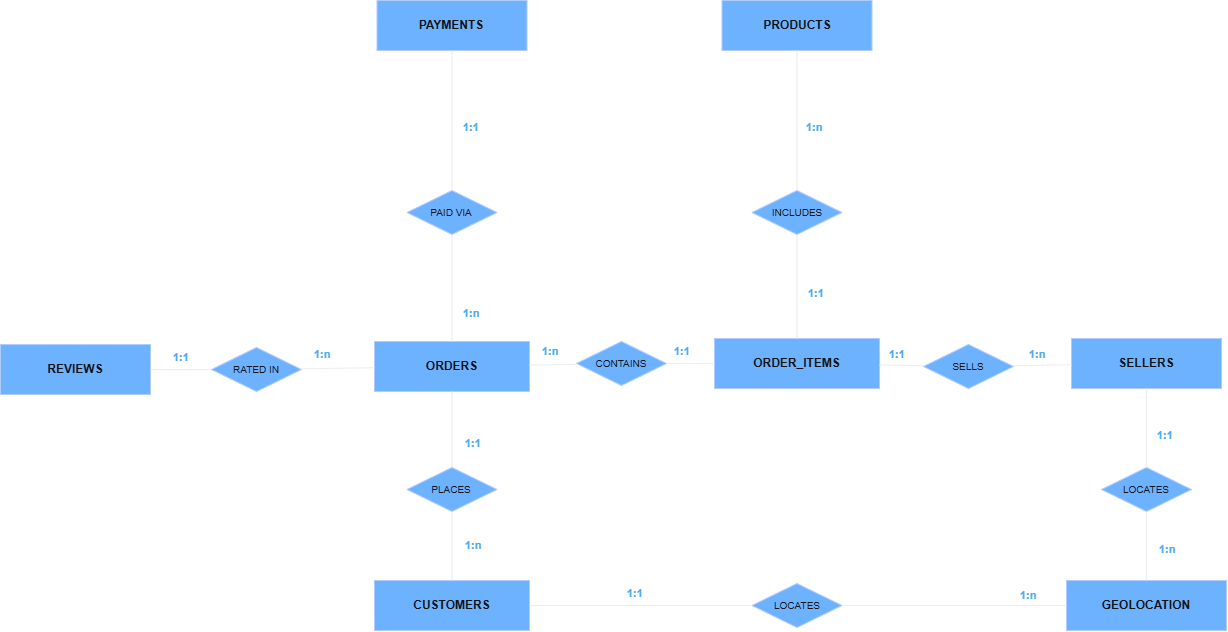
\includegraphics[width=\textwidth]{er_schema_pieno.png}
  \caption{Schema E/R del Reconciled Database}
  \label{fig:er}
\end{figure}

\subsection{Schema Relazionale}

Di seguito lo schema relazionale (chiavi primarie sottolineate; asterisco = chiave
esterna):

\begin{itemize}
  \item \textbf{Customers}(\underline{customer\_id}, customer\_unique\_id,
        zip\_code\_prefix*, city, state)\\
        \textit{\texttt{customer\_unique\_id} identifica il cliente reale: uno stesso
        cliente può avere più \texttt{customer\_id} su ordini distinti.
        \texttt{zip\_code\_prefix} è FK parziale/opzionale verso \texttt{Geolocation}
        (278 record cliente, pari a 157 CAP distinti, senza corrispondenza nella tabella di geolocalizzazione; join eseguito come LEFT JOIN).}

  \item \textbf{Sellers}(\underline{seller\_id}, zip\_code\_prefix*, city, state)\\
        \textit{\texttt{zip\_code\_prefix} è FK parziale/opzionale verso \texttt{Geolocation}
        (7 CAP venditori assenti; join eseguito come LEFT JOIN).}

  \item \textbf{Products}(\underline{product\_id}, category\_name,
        category\_name\_english, name\_length, description\_length, photos\_qty,
        weight\_g, length\_cm, height\_cm, width\_cm)\\
        \textit{\texttt{category\_name\_english} è attributo derivato dal join con la
        tabella di traduzione.}

  \item \textbf{Orders}(\underline{order\_id}, customer\_id*, status,
        purchase\_timestamp, approved\_at, delivered\_carrier\_date,
        delivered\_customer\_date, estimated\_delivery\_date,
        delivery\_lead\_days, delivery\_delay\_days)\\
        \textit{\texttt{delivery\_lead\_days} e \texttt{delivery\_delay\_days} sono
        calcolati in fase di cleaning. Sono NULL per ordini non ancora consegnati;
        questa condizione è tracciata da appositi flag binari.}

  \item \textbf{Order\_Items}(\underline{order\_id*, order\_item\_id}, product\_id*,
        seller\_id*, shipping\_limit\_date, price, freight\_value)\\
        \textit{Chiave primaria composta: un ordine può contenere più prodotti.}

  \item \textbf{Payments}(\underline{order\_id*, payment\_sequential},
        payment\_type, installments, value)\\
        \textit{Un ordine può avere più metodi di pagamento, da cui la chiave composta
        con \texttt{payment\_sequential}.}

  \item \textbf{Reviews}(\underline{review\_id}, order\_id*, score, comment\_title,
        comment\_message, creation\_date, answer\_timestamp)\\
        \textit{Il punteggio è un intero da 1 a 5. I campi testo sono facoltativi.}

  \item \textbf{Geolocation}(\underline{zip\_code\_prefix}, lat, lng, city, state)\\
        \textit{Mappa ogni prefisso postale a un centroide geografico. Risultato
        dell'aggregazione per ZIP effettuata in cleaning.}
\end{itemize}

% ═══════════════════════════════════════════════════════════════════════════
%  3. DATA QUALITY ASSESSMENT E DATA CLEANING
% ═══════════════════════════════════════════════════════════════════════════
\section{Data Quality Assessment e Data Cleaning}

\subsection{Metodologia}

Le operazioni di pulizia sono state implementate in un notebook Python
(\texttt{olist\_dw\_cleaning\_pipeline.ipynb}), strutturato come una pipeline
modulare e auditabile. Ogni fase di trasformazione registra un entry nell'audit log
globale, che traccia per ogni step: tabella, operazione, righe prima/dopo, numero di
modifiche e note esplicative.

Il processo ha seguito le fasi dello standard di data quality assessment adottato a
lezione: \textbf{analisi dei dati grezzi} (profiling), \textbf{identificazione dei
problemi} con scorecard programmatica, \textbf{classificazione} secondo la tassonomia
del corso e \textbf{intervento correttivo}, seguito dalla verifica dei risultati.

\subsubsection*{Classificazione dei problemi di data quality}

Secondo la tassonomia adottata nel corso, i problemi di qualità dei dati si
distinguono in:

\begin{itemize}
\sloppy
  \item \textbf{Missing values}: valori assenti che devono essere presenti per garantire
        la completezza del dato. Da distinguere dai \textit{null semantici}, che sono
        assenze legittime (es.\ data di consegna per ordini non ancora consegnati).
  \item \textbf{Wrong values}: valori presenti ma scorretti rispetto al dominio atteso
        (es.\ \texttt{customer\_zip\_code\_prefix} troncato a 4 cifre per perdita
        dello zero iniziale, coordinate fuori range geografico).
  \item \textbf{Noisy data}: valori plausibili ma anomali rispetto alla distribuzione
        statistica, non rilevabili da regole di dominio semplici. Richiedono analisi
        della distribuzione (es.\ varianza/deviazione standard, media~$\pm 3\sigma$).
  \item \textbf{Violations of attribute dependencies}: valori che violano dipendenze
        funzionali tra attributi dello stesso record (es.\ \texttt{approved\_at} $<$
        \texttt{purchase\_timestamp}).
  \item \textbf{Record duplication}: più record che rappresentano la stessa entità
        reale, con o senza differenze di valore.
  \item \textbf{Varying value representations}: lo stesso concetto rappresentato con
        formati diversi (es.\ ``são paulo'' vs.\ ``São Paulo'').
\end{itemize}

\subsubsection*{Indici di data quality}

Per ogni dataset sono stati misurati i seguenti cinque indici di qualità:

\begin{itemize}
  \item \textbf{Validity}: percentuale di valori che rispettano le regole di dominio
        dichiarate (tipo, range, whitelist). Calcolata per attributo.
  \item \textbf{Completeness}: percentuale di valori non nulli sugli attributi
        obbligatori. Non include attributi facoltativi per non falsare l'indice.
  \item \textbf{Uniqueness}: percentuale di record non duplicati sulla chiave primaria.
  \item \textbf{Consistency}: percentuale di record che rispettano le dipendenze
        funzionali inter-attributo dichiarate.
  \item \textbf{Precision}: percentuale di dati corretti, ovvero non anomali
        statisticamente. Per colonne numeriche è calcolata come percentuale di
        valori entro media~$\pm 3\sigma$; per tabelle senza colonne numeriche
        rilevanti, Precision è assunta al 100\%.
\end{itemize}

Gli indici sono calcolati automaticamente da una \textbf{scorecard programmatica}
(classe \texttt{DQAReport}), basata su regole dichiarative per ciascun attributo
(lambda Python per Validity, lista attributi obbligatori per Completeness, chiave per
Uniqueness, lista di dipendenze per Consistency). La scorecard fornisce una vista
oggettiva e riproducibile della qualità, ma non è sufficiente da sola: i
\textit{noisy data} non emergono dagli indici di Validity se le regole sono permissive
(es.\ \texttt{price > 0}), e richiedono un'ispezione aggiuntiva delle distribuzioni
statistiche.

\begin{aibox}{Data Quality Assessment (L1) -- \texttt{10\_script\_llm}}
A supporto dell'interpretazione dei risultati della scorecard è stato utilizzato
un Large Language Model (\texttt{llama3.2:3b} via Ollama, locale) come strumento
di analisi narrativa. Per ogni tabella, dopo aver calcolato il profilo statistico
con pandas (null per colonna, duplicati, statistiche numeriche min/max/mean), il
prompt inviato al modello era: \textit{``Analizza la qualità dei dati di questa
tabella Olist:''} seguito dal profilo calcolato.
Il LLM ha prodotto per ogni tabella una descrizione in linguaggio naturale dei
problemi rilevati, con una spiegazione del perché ciascun problema impatta il
Data Warehouse e un suggerimento operativo. Questo ha supportato le decisioni
di intervento descritte nei paragrafi seguenti, nei casi in cui la scorecard da
sola non era sufficiente a spiegare la natura del problema.
\end{aibox}

La Tabella~\ref{tab:raw} riepiloga le dimensioni delle tabelle sorgente prima di
qualsiasi intervento.

\begin{table}[H]
  \centering
  \caption{Dimensioni delle tabelle sorgente (dati grezzi)}
  \label{tab:raw}
  \begin{tabular}{lrrr}
    \toprule
    \textbf{Tabella} & \textbf{Righe} & \textbf{Missing totali} & \textbf{Duplicati esatti} \\
    \midrule
    Customers    &   99.441 &       0 &       0 \\
    Sellers      &    3.095 &       0 &       0 \\
    Products     &   32.951 &   2.448 &       0 \\
    Orders       &   99.441 &   4.908 &       0 \\
    Order Items  &  112.650 &       0 &       0 \\
    Payments     &  103.886 &       0 &       0 \\
    Reviews      &   99.224 & 145.903 &       0 \\
    Geolocation  & 1.000.163 &      0 & 261.831 \\
    \bottomrule
  \end{tabular}
\end{table}

\subsection{Problemi rilevati e interventi}

\subsubsection{Customers (99.441 record)}

\begin{figure}[H]
  \centering
  
\includegraphics[width=0.9\textwidth]{dq_plot_customers.png}
  \caption{Data quality assessment -- \texttt{olist\_customers\_dataset}}
  \label{fig:dq_customers}
\end{figure}

Completeness, Uniqueness e Consistency sono al 100\%. Lo scorecard rileva un
problema di \textbf{Validity} (75,87\%), interamente attribuibile alla colonna
\texttt{customer\_zip\_code\_prefix}: la regola di dominio richiede un CAP numerico a
5 cifre, ma 23.995 record su 99.441 (24,1\%) presentano un CAP a 4 cifre, perché il
CSV originale memorizza il campo come numero e perde lo zero iniziale dei CAP che
iniziano per \texttt{0} (\textit{wrong values}). La colonna \texttt{customer\_state}
risulta invece già conforme alla whitelist \texttt{BR\_STATES} (0 record invalidi):
nel CSV originale i codici di stato sono già tutti in maiuscolo.

Un'ispezione manuale rivela inoltre un secondo problema, non catturato dallo
scorecard perché \texttt{customer\_city} non è soggetto a regole di dominio: la
presenza di \textbf{varying value representations} sui nomi di città (es.\
``são paulo'' vs.\ ``São Paulo''). Si tratta di un errore a livello di istanza
classificabile come problema di \textbf{Consistency}, gestito a parte rispetto allo
scorecard.

\textbf{Intervento -- automatic correction:} \texttt{str.strip()} su tutti i campi
testo per rimuovere spazi superflui; \texttt{str.title()} su
\texttt{customer\_city} (Consistency); \texttt{str.upper()} su
\texttt{customer\_state} applicato in via cautelativa per garantire l'invarianza
rispetto al maiuscolo/minuscolo (0 modifiche effettive, poiché i valori erano già
tutti conformi a \texttt{BR\_STATES}).

\textbf{Risultato}: 99.441 record, 0 missing, 0 duplicati; Completeness, Uniqueness e
Consistency al 100\%. Il problema di Validity sul \texttt{customer\_zip\_code\_prefix}
(CAP a 4 cifre) non viene corretto dalla pipeline: resta documentato come limite noto
della qualità del dato, senza impatto sulle analisi a livello città/stato.

\subsubsection{Sellers (3.095 record)}

\begin{figure}[H]
  \centering
  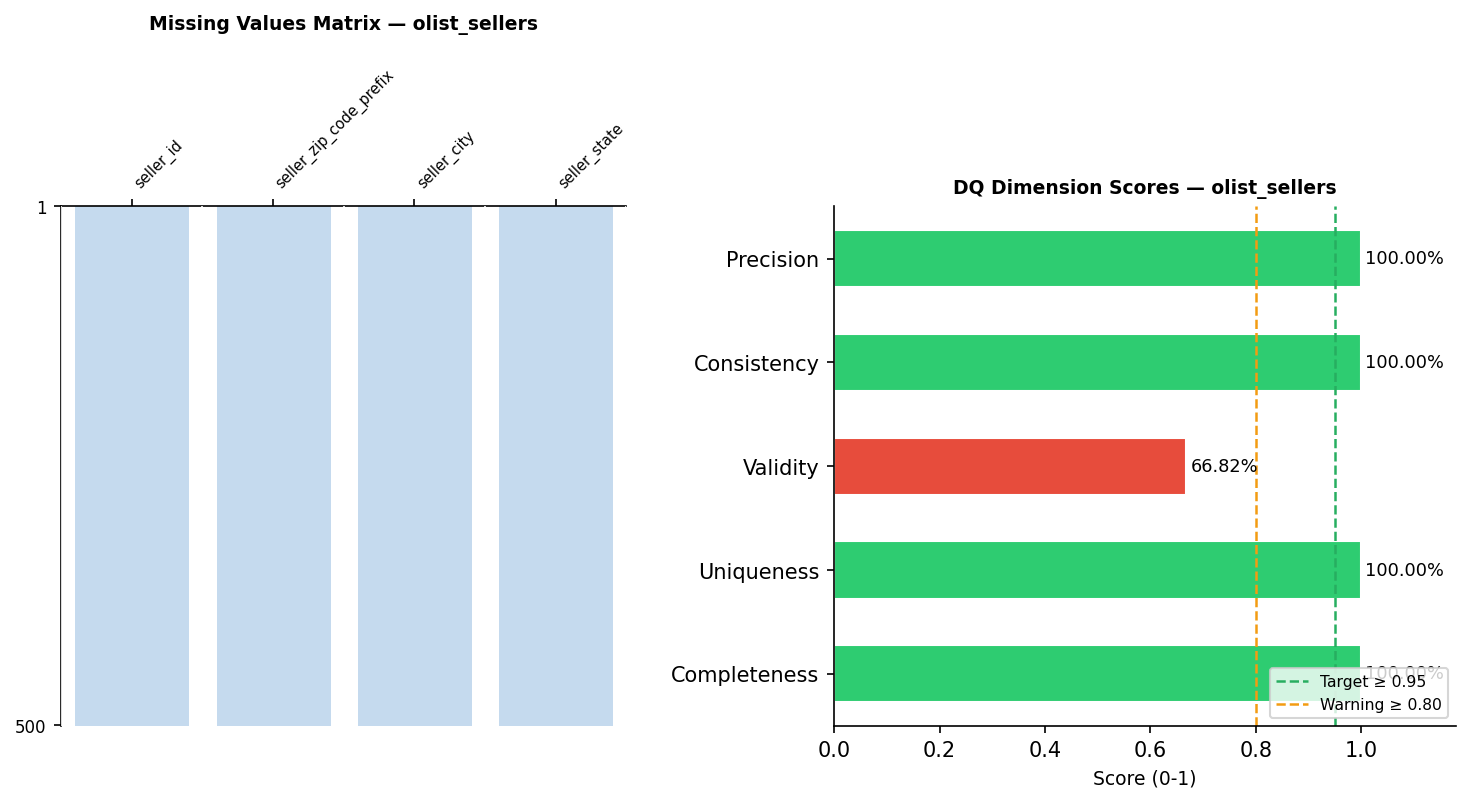
\includegraphics[width=0.9\textwidth]{dq_plot_sellers.png}
  \caption{Data quality assessment -- \texttt{olist\_sellers\_dataset}}
  \label{fig:dq_sellers}
\end{figure}

Situazione analoga a customers: lo scorecard rileva un problema di \textbf{Validity}
(66,82\%), causato dalla colonna \texttt{seller\_zip\_code\_prefix}: 1.027 record su
3.095 (33,2\%) presentano un CAP a 4 cifre per lo stesso motivo (perdita dello zero
iniziale nel CSV originale). La colonna \texttt{seller\_state} è già conforme alla
whitelist \texttt{BR\_STATES} (0 record invalidi): anche per i sellers i codici di
stato sono già tutti in maiuscolo nel CSV originale. L'ispezione manuale rileva
inoltre il problema di Consistency sulle \textit{varying value representations} di
\texttt{seller\_city}.

\textbf{Intervento -- automatic correction:} \texttt{str.strip()} e
\texttt{str.title()} su \texttt{seller\_city} (Consistency); \texttt{str.upper()} su
\texttt{seller\_state} applicato in via cautelativa (0 modifiche effettive, valori
già conformi a \texttt{BR\_STATES}).

\textbf{Risultato}: 3.095 record, 0 missing, 0 duplicati; Completeness, Uniqueness e
Consistency al 100\%. Come per customers, il problema di Validity sul
\texttt{seller\_zip\_code\_prefix} (CAP a 4 cifre) resta un limite noto, documentato
ma non corretto dalla pipeline.

\subsubsection{Geolocation (1.000.163 record originali)}

\begin{figure}[H]
  \centering
  
\includegraphics[width=0.9\textwidth]{dq_plot_geolocation.png}
  \caption{Data quality assessment -- \texttt{olist\_geolocation\_dataset}}
  \label{fig:dq_geo}
\end{figure}

Lo scorecard evidenzia due problemi principali. Il primo è di \textbf{Uniqueness}
(58,84\%): il dataset registra più coordinate per lo stesso prefisso postale, con
261.831 righe duplicate (26,2\%). Si tratta di \textit{record duplication}: più record
rappresentano la stessa entità reale con valori diversi. Il secondo problema è di
\textbf{Validity} (75,43\%): alcune righe presentano coordinate \texttt{lat}/\texttt{lng}
fuori dal range geografico del Brasile ($lat \in [-33.75; 5.27]$,
$lng \in [-73.99; -34.79]$), classificabili come \textit{wrong values}.

\textbf{Interventi:}
\begin{enumerate}
  \item Normalizzazione testuale di \texttt{city} e \texttt{state} -- automatic
        correction (Consistency).
  \item Filtraggio dei record con coordinate fuori range -- automatic correction
        (Validity).
  \item Rimozione dei duplicati esatti con \texttt{drop\_duplicates()} (Uniqueness).
  \item Aggregazione per \texttt{zip\_code\_prefix}: media di lat/lng (centroide),
        moda di city/state, mantenendo in \texttt{n\_records} il conteggio dei
        punti originali aggregati per ciascun prefisso (utile come indicatore
        di affidabilità del centroide).
\end{enumerate}

\textbf{Risultato}: 19.015 record, 0 missing, 0 duplicati.

\subsubsection{Products (32.951 record)}

\begin{figure}[H]
  \centering
  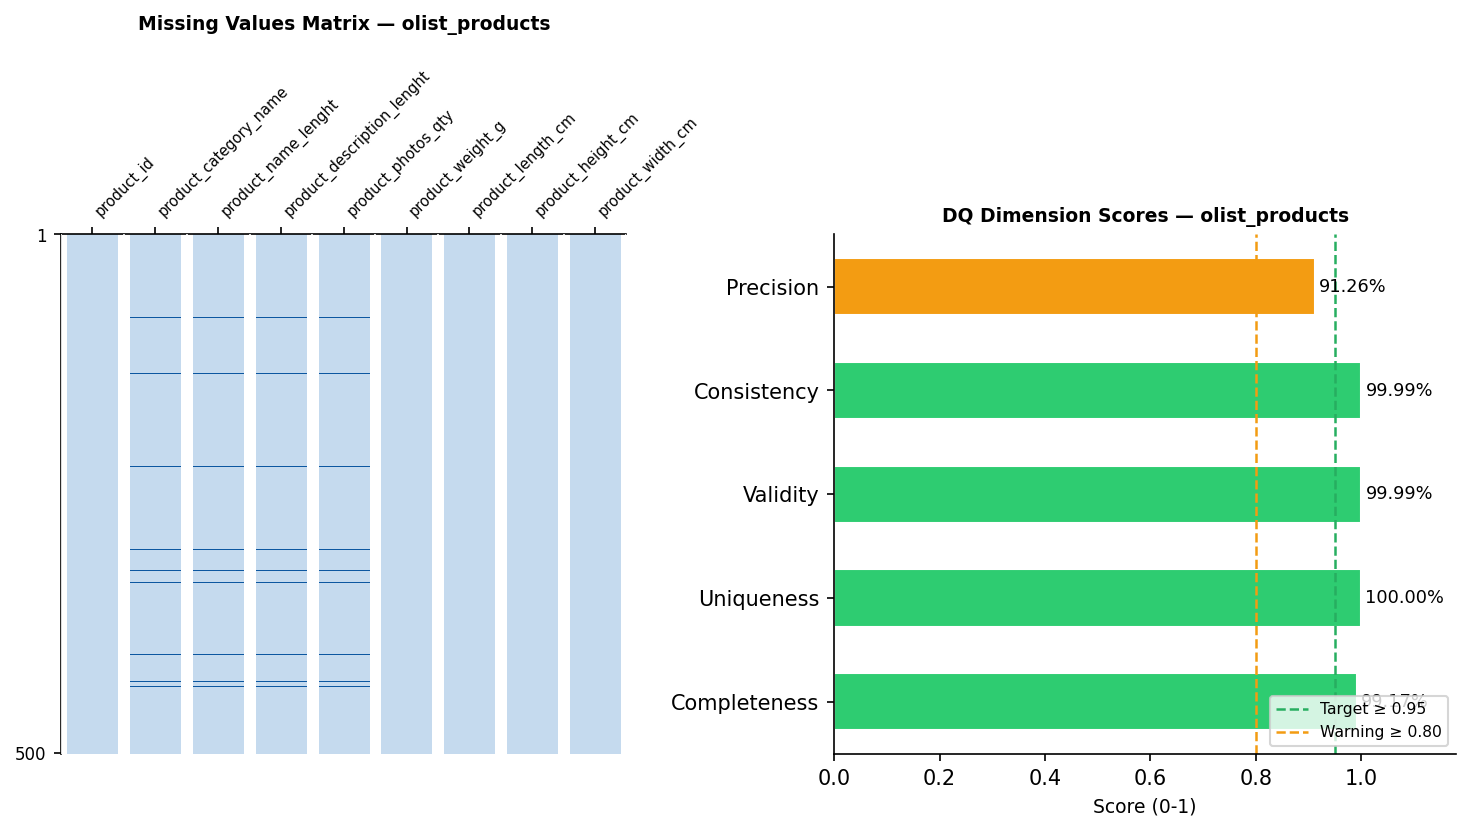
\includegraphics[width=0.9\textwidth]{dq_plot_products.png}
  \caption{Data quality assessment -- \texttt{olist\_products\_dataset}}
  \label{fig:dq_products}
\end{figure}

Lo scorecard mostra \textbf{Completeness} a 99,17\%, dovuta a 610 valori mancanti in
\texttt{product\_category\_name} (1,85\%) e a valori nulli nelle colonne fisiche
(peso, dimensioni). Validity, Uniqueness e Consistency sono prossime al 100\%.

L'analisi della distribuzione delle misure fisiche rivela inoltre un problema di
\textit{noisy data} non rilevato dallo scorecard: la regola di Validity impone solo
\texttt{> 0}, e quindi i valori plausibili ma anomali (peso $= 40.000\,\text{g}$,
dimensioni estreme) passano il check. Questi outlier costituiscono comunque un
problema da trattare, classificabile come \textit{noisy data / wrong values} secondo
la classificazione del corso, anche se rimangono ``invisibili'' alla scorecard.

Da notare che i nomi di colonna \texttt{product\_name\_lenght} e
\texttt{product\_description\_lenght} (typo nella sorgente: manca la ``h'') sono
stati mantenuti tali quali per compatibilità con lo schema originale.

\begin{aibox}{Missing Values \& Outlier Classification (L2) -- \texttt{10\_script\_llm}}
Per la classificazione dei valori mancanti è stato usato il LLM come supporto.
Il prompt inviato al modello era: \textit{``Per ogni colonna: classifica
MCAR/MAR/MNAR con motivazione, impatto sul DW, strategia raccomandata.''},
preceduto dai dati di missingness calcolati con pandas (numero di null e
percentuale per colonna).
Il modello ha spiegato che i null in \texttt{product\_category\_name} sono
classificabili come \textbf{MCAR} (Missing Completely At Random): l'assenza
non è correlata ad altri attributi ma riflette prodotti non catalogati dal
venditore al momento dell'inserimento, senza un pattern sistematico. Ha quindi
indicato il \textit{fill in} con costante globale (\texttt{"unknown"}) come
strategia raccomandata, in quanto non introduce bias e preserva la riga nel
dataset. Per le misure fisiche, ha suggerito l'imputazione con la mediana di
colonna, più robusta della media in presenza di outlier.
\end{aibox}

\textbf{Interventi:}
\begin{enumerate}
  \item \textbf{Missing values} su \texttt{product\_category\_name}
        (Completeness): \textit{fill in} automaticamente con la costante globale
        \texttt{"unknown"}, poiché non è possibile inferire la categoria corretta
        senza informazioni aggiuntive (tecnica vista a lezione:
        \textit{fill in with a global constant}).

  \item \textbf{Missing values} nelle colonne numeriche fisiche (Completeness):
        \textit{fill in} automaticamente con la \textbf{mediana dell'attributo}
        calcolata sui record validi. Le slide del corso indicano la media come
        opzione standard; ho scelto la mediana perché più robusta in presenza di
        outlier. Per ogni colonna imputata è stato aggiunto un flag binario
        \texttt{\_imputed}.

  \item \textbf{Noisy data} nelle colonne fisiche: rilevamento tramite metodo
        \textbf{IQR} (\textit{Interquartile Range}: soglia inferiore $Q_1 - 1.5 \cdot IQR$,
        soglia superiore $Q_3 + 1.5 \cdot IQR$);
        flag binario \texttt{\_outlier} aggiunto per ogni colonna, valori originali
        preservati nel reconciled database.

  \item Join con la tabella di traduzione per aggiungere
        \texttt{product\_category\_name\_english}.
\end{enumerate}

\textbf{Risultato}: 32.951 record, 0 missing, 0 duplicati. La tabella include 22
colonne (9 originali $+$ colonna EN $+$ 12 flag: 8 flag \texttt{\_imputed} e 4 flag
\texttt{\_outlier}).

\subsubsection{Orders (99.441 record)}
\label{sec:orders-cleaning}

\begin{figure}[H]
  \centering
  
\includegraphics[width=0.9\textwidth]{dq_plot_orders.png}
  \caption{Data quality assessment -- \texttt{olist\_orders\_dataset}}
  \label{fig:dq_orders}
\end{figure}

Lo scorecard mostra \textbf{Completeness} a 99,38\% e \textbf{Consistency} a 96,98\%,
mentre Validity e Uniqueness sono al 100\%. La Precision è al 100\% per questa
tabella, in quanto non sono presenti colonne numeriche con distribuzioni anomale
rilevanti; i problemi di noisy data per Orders riguardano le colonne temporali,
già gestite tramite flag per i null semantici.

I valori nulli nelle colonne temporali (160 in \texttt{order\_approved\_at}, 1.783
in \texttt{order\_delivered\_carrier\_date}, 2.965 in
\texttt{order\_delivered\_customer\_date}) sono \textbf{semanticamente corretti}:
corrispondono a ordini non approvati o non ancora consegnati. Non si tratta di veri
missing values e non devono essere imputati. Il calo di Consistency (96,98\%) è
dovuto a 3.003 record che violano almeno una delle dipendenze tra date
(es.\ \texttt{approved\_at} $<$ \texttt{purchase\_timestamp}) -- problema
classificabile come \textit{violated attribute dependencies} a livello di record.

\textbf{Interventi:}
\begin{enumerate}
  \item \texttt{str.lower()} su \texttt{order\_status} -- automatic correction
        (Consistency a livello di rappresentazione).
  \item \texttt{pd.to\_datetime()} su tutte le colonne temporali -- automatic
        correction (Validity: i timestamp erano memorizzati come stringhe anziché
        come date).
  \item Flag binari \texttt{\_approved\_missing}, \texttt{\_delivered\_carrier\_missing},
        \texttt{\_delivered\_customer\_missing} per tracciare i null semantici senza
        imputarli.
  \item Le violazioni di dipendenza tra date vengono mantenute nel reconciled database
        con i timestamp originali (non imputate), ma tracciate per successive analisi.
  \item Feature engineering:
        \begin{itemize}
          \item \texttt{delivery\_delay\_days} $=$ consegna effettiva $-$ consegna
                stimata (negativo $=$ anticipo);
          \item \texttt{delivery\_lead\_days} $=$ consegna effettiva $-$ data
                acquisto;
          \item \texttt{purchase\_year}, \texttt{purchase\_month} estratti dal
                timestamp di acquisto.
        \end{itemize}
\end{enumerate}

\textbf{Risultato}: 99.441 record, 0 duplicati. Rimangono \texttt{NaN} nelle colonne
derivate per gli ordini non consegnati (previsto). 15 colonne totali.

\subsubsection{Order Items (112.650 record)}

\begin{figure}[H]
  \centering
  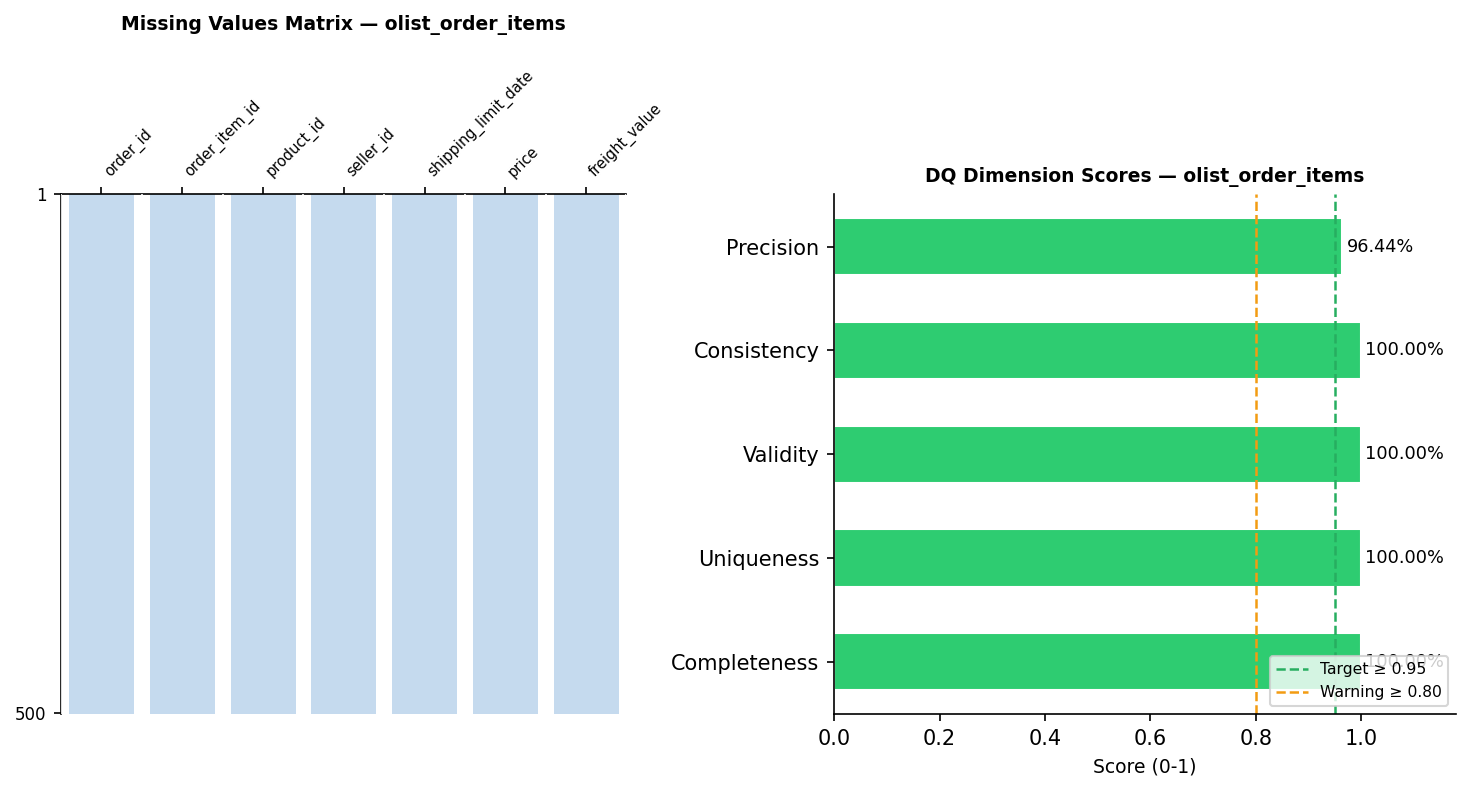
\includegraphics[width=0.9\textwidth]{dq_plot_order_items.png}
  \caption{Data quality assessment -- \texttt{olist\_order\_items\_dataset}}
  \label{fig:dq_items}
\end{figure}

Lo scorecard mostra Completeness, Uniqueness, Validity e Consistency tutte al 100\%.
La Precision è calcolata sulla colonna \texttt{price}: misura la percentuale di
valori entro media~$\pm 3\sigma$, identificando i potenziali noisy data.

L'analisi della distribuzione di \texttt{price} rivela un problema di
\textit{noisy data} non rilevato dallo scorecard: la regola di Validity impone solo
\texttt{price > 0}, e i valori sono tutti positivi, ma la distribuzione
si estende fino a 6.735 BRL con una coda destra molto allungata. Stessa situazione
per \texttt{freight\_value}. Si tratta di un classico esempio di problema visibile
dall'analisi della distribuzione ma non da una regola puntuale, classificabile come
\textit{noisy data / wrong values} secondo la tassonomia del corso.

\textbf{Interventi:}
\begin{enumerate}
  \item \texttt{pd.to\_datetime()} su \texttt{shipping\_limit\_date} -- automatic
        correction (Validity).
  \item \textbf{Noisy data} su \texttt{price}: rilevamento tramite metodo
        \textbf{IQR} ($Q_1 - 1.5 \cdot IQR$ / $Q_3 + 1.5 \cdot IQR$).
        Flag binario \texttt{\_price\_outlier} aggiunto. Valori originali preservati.
  \item \textbf{Noisy data} su \texttt{freight\_value}: stessa metodologia di
        \texttt{price}. Flag \texttt{\_freight\_value\_outlier}. Valori originali preservati.
\end{enumerate}

\begin{figure}[H]
  \centering
  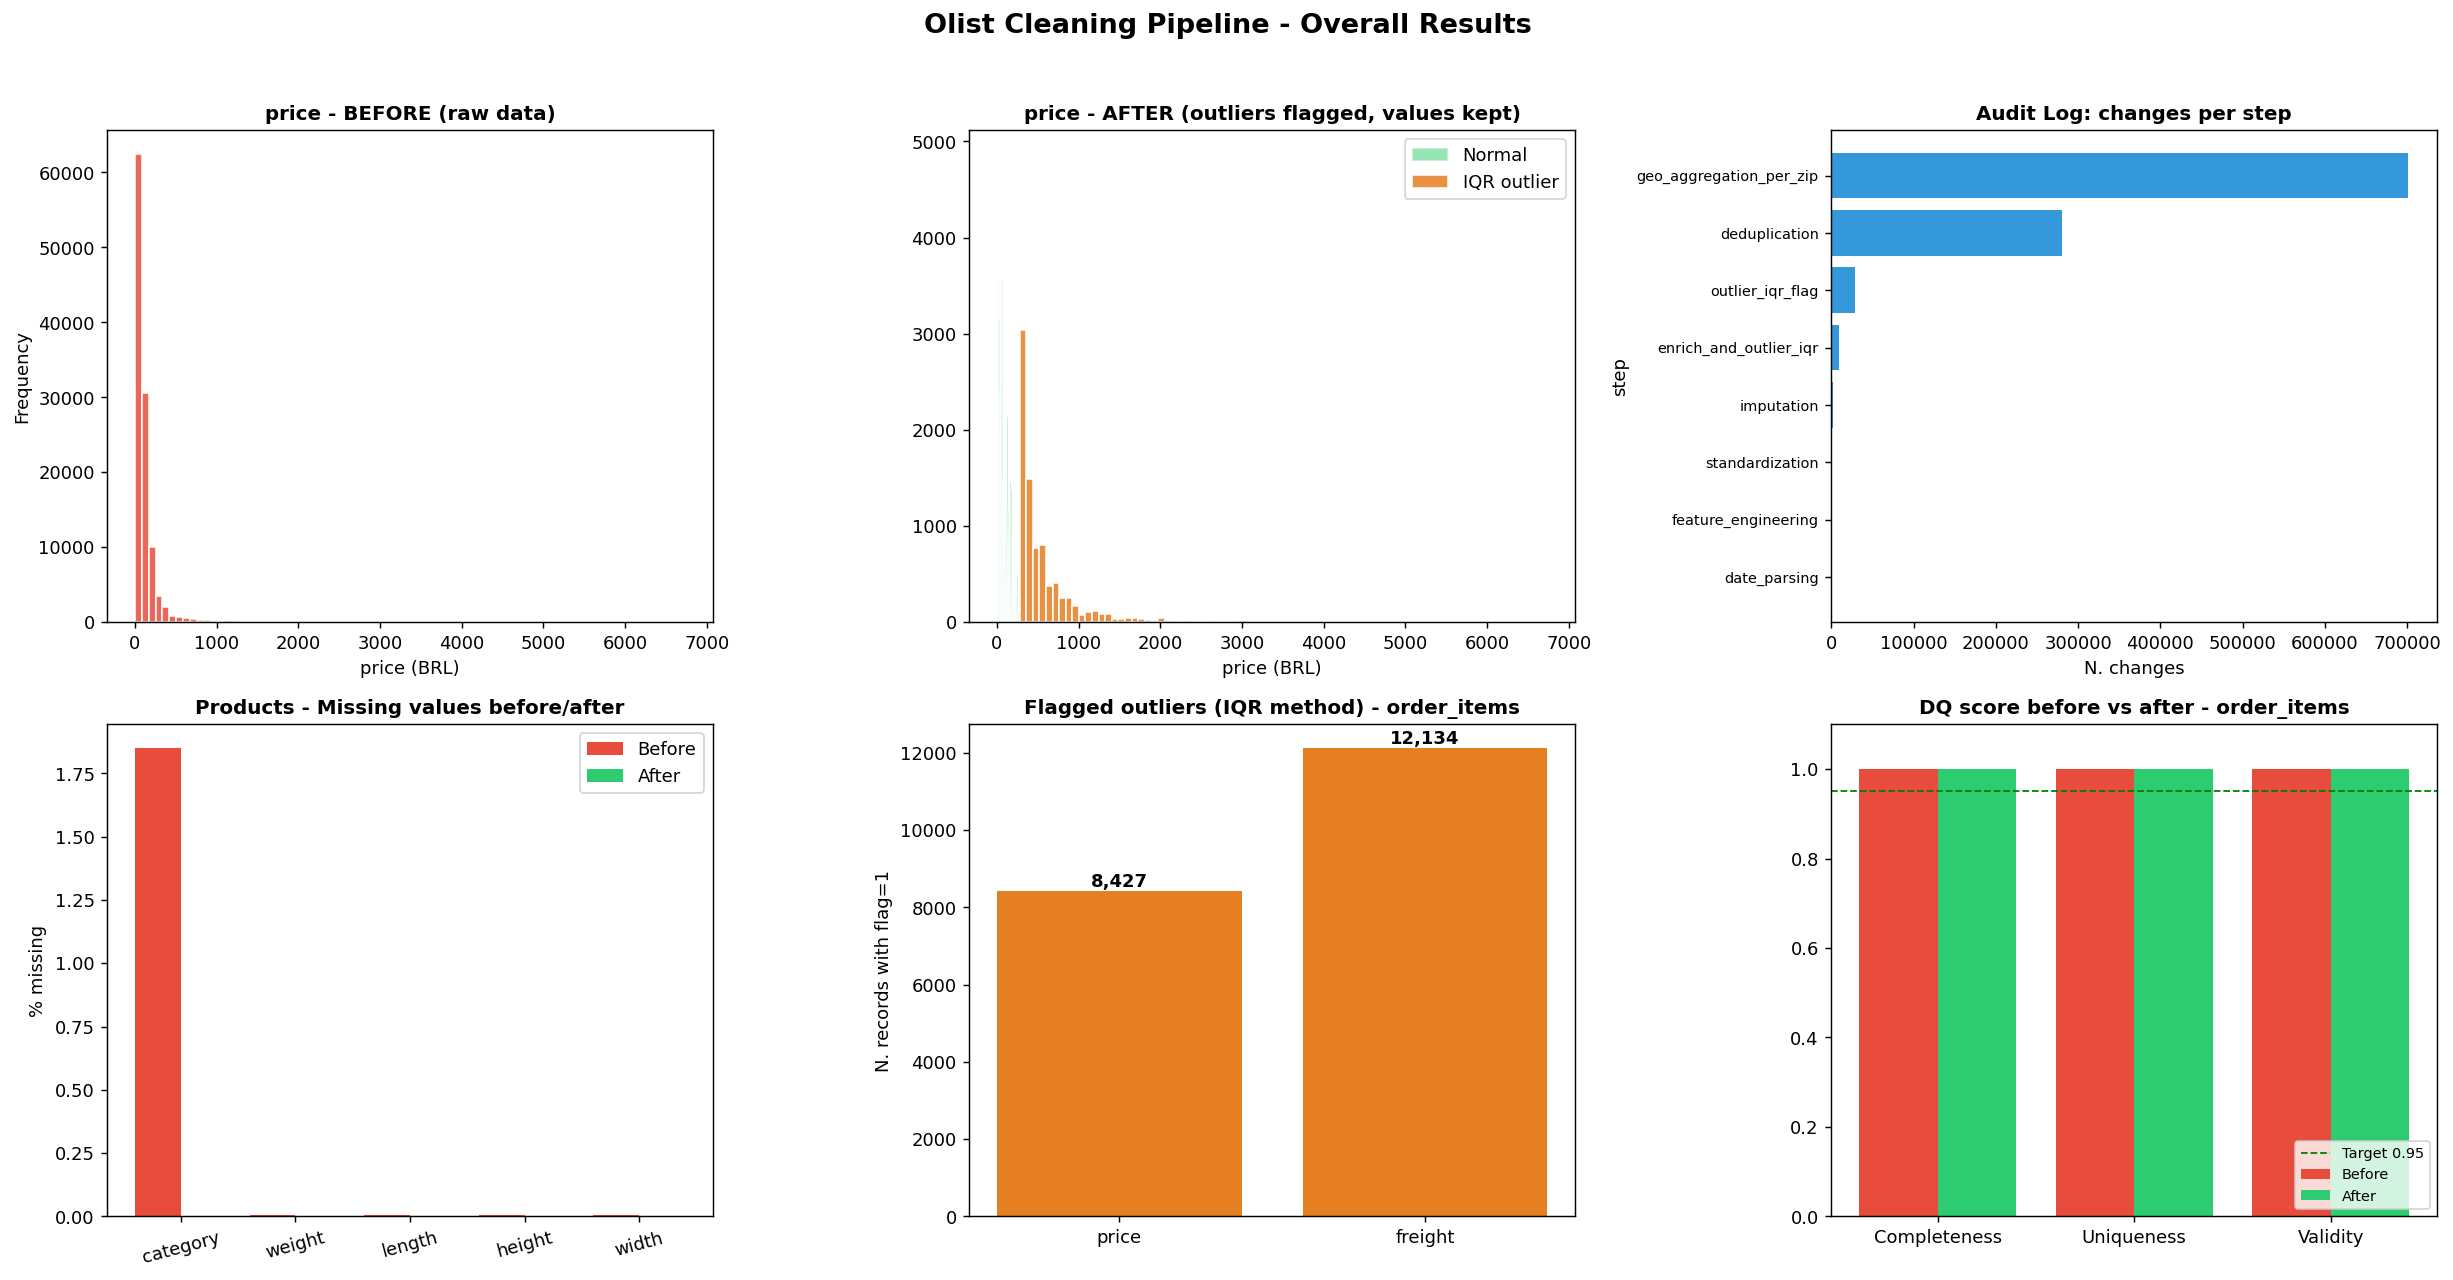
\includegraphics[width=\textwidth]{cleaning_pipeline_results.png}
  \caption{Risultati complessivi della cleaning pipeline: distribuzione \texttt{price}
           prima/dopo, audit log per step, missing values Products, outlier flaggati
           (metodo IQR) per \texttt{order\_items} e DQ score prima/dopo.}
  \label{fig:pipeline}
\end{figure}

\textbf{Risultato}: 112.650 record, 0 missing, 0 duplicati. 9 colonne (7 originali
$+$ 2 flag \texttt{\_outlier}).

\textit{Nota: \texttt{total\_item\_value} $=$ \texttt{price} $+$ \texttt{freight\_value}
non è stata aggiunta nel reconciled database perché è una misura derivata semplice;
viene calcolata direttamente in Tableau durante la visualizzazione.}

\subsubsection{Payments (103.886 record)}

\begin{figure}[H]
  \centering
  
\includegraphics[width=0.9\textwidth]{dq_plot_order_payments.png}
  \caption{Data quality assessment -- \texttt{olist\_order\_payments\_dataset}}
  \label{fig:dq_payments}
\end{figure}

Lo scorecard mostra tutti gli indici al 100\%. Il campo \texttt{payment\_type} ha
cinque valori: \texttt{credit\_card} (76.795, 73,9\%), \texttt{boleto} (19.784,
19,0\%), \texttt{voucher} (5.775, 5,6\%), \texttt{debit\_card} (1.529, 1,5\%) e
\texttt{not\_defined} (3 record, 0,003\%). I tre record \texttt{not\_defined} sono
ammessi nella whitelist di Validity perché il numero è trascurabile e potrebbero
essere transazioni legittime non classificate.

Anche qui, l'analisi della distribuzione di \texttt{payment\_value} evidenzia un
problema di \textit{noisy data} che la regola \texttt{>= 0} non cattura: sono
presenti valori molto elevati nella coda destra. Lo trattiamo come per i prezzi degli
order items.

\textbf{Interventi:}
\begin{enumerate}
  \item \texttt{str.lower()} su \texttt{payment\_type} -- automatic correction
        (Consistency a livello di rappresentazione).
  \item \textbf{Noisy data} su \texttt{payment\_value}: rilevamento tramite metodo
        \textbf{IQR} ($Q_1 - 1.5 \cdot IQR$ / $Q_3 + 1.5 \cdot IQR$) $+$ flag
        \texttt{\_payment\_value\_outlier}. Valori originali preservati.
\end{enumerate}

\textbf{Risultato}: 103.886 record, 0 missing, 0 duplicati. 6 colonne (5 originali
$+$ 1 flag \texttt{\_payment\_value\_outlier}).

\subsubsection{Reviews (99.224 record dopo cleaning)}

\begin{figure}[H]
  \centering
  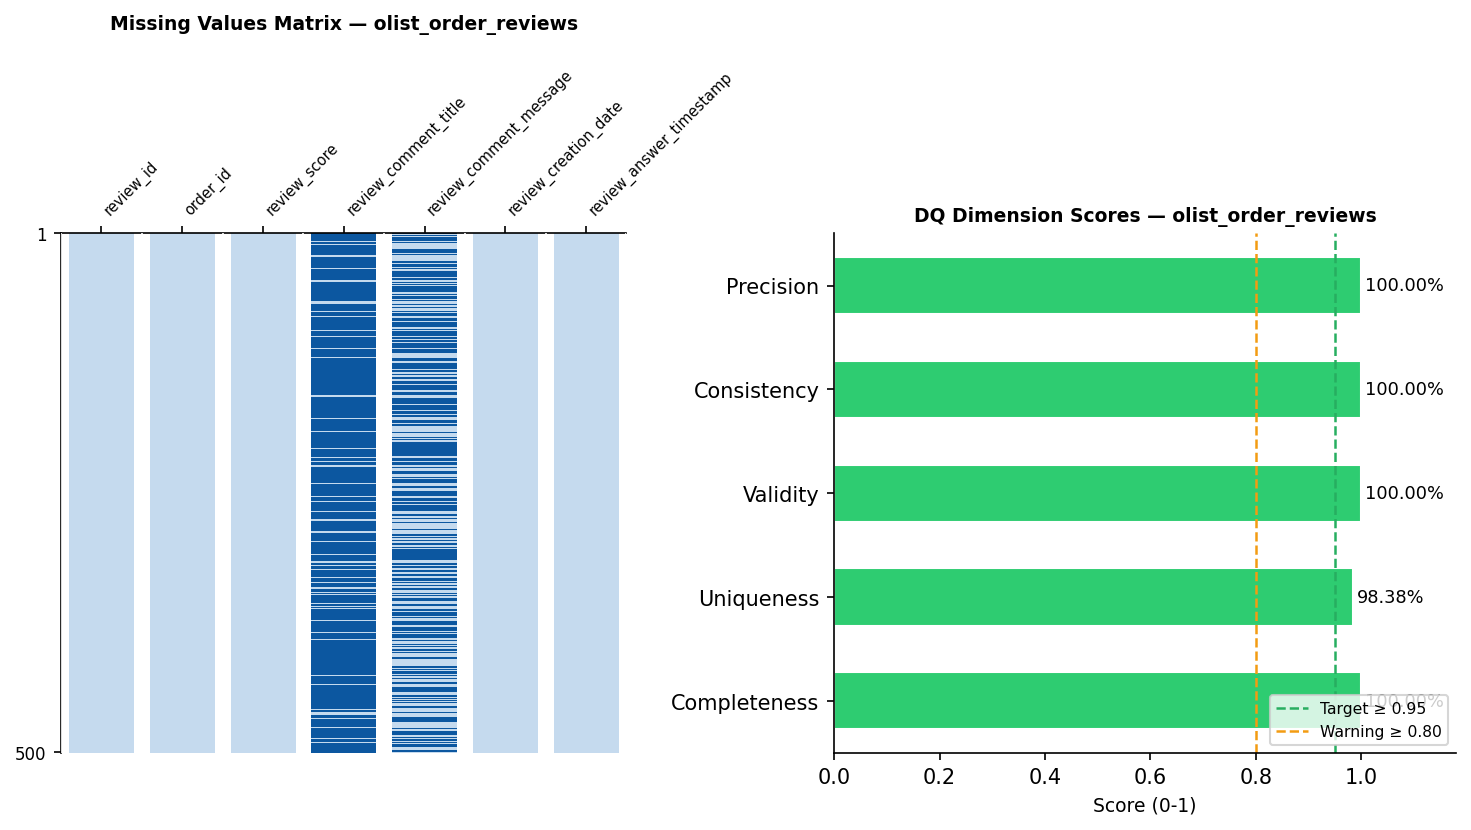
\includegraphics[width=0.9\textwidth]{dq_plot_order_reviews.png}
  \caption{Data quality assessment -- \texttt{olist\_order\_reviews\_dataset}}
  \label{fig:dq_reviews}
\end{figure}

Lo scorecard, calcolato assumendo \texttt{review\_id} come chiave primaria, mostra
\textbf{Uniqueness} al 98,38\% (1.603 record con \texttt{review\_id} ripetuto, di
cui 814 eccedenti la prima occorrenza), mentre Validity e Completeness sono al
100\%.

Un'analisi più approfondita mostra però che questi record non sono duplicati:
i 1.603 record con \texttt{review\_id} ripetuto corrispondono a 789 valori di
\texttt{review\_id} ciascuno associato a 2 o più \texttt{order\_id} distinti (lo
stesso punteggio/commento del cliente viene replicato su più ordini, ad es. ordini
multipli o sostituzioni). Sulla chiave composta (\texttt{review\_id},
\texttt{order\_id}) non esiste invece alcun duplicato: tutti i 99.224 record sono
univoci su questa coppia. La chiave naturale corretta per questa tabella è quindi
(\texttt{review\_id}, \texttt{order\_id}) e non il solo \texttt{review\_id}; lo
scorecard, basato su una chiave a singolo attributo, sovrastima la duplicazione
reale.

È importante notare che il check di Completeness è stato applicato solo agli
attributi obbligatori (\texttt{review\_id}, \texttt{order\_id}, \texttt{review\_score},
\texttt{review\_creation\_date}, \texttt{review\_answer\_timestamp}) ed esclude i
due campi facoltativi \texttt{review\_comment\_title} e
\texttt{review\_comment\_message}.

I null in \texttt{review\_comment\_title} (87.656, 88,3\%) e
\texttt{review\_comment\_message} (58.247, 58,7\%) sono infatti semanticamente
corretti: il commento scritto è facoltativo. Includerli nel check di Completeness
avrebbe falsato l'indice, perché i null in questi campi non sono ``dati mancanti''
ma ``dati assenti per scelta dell'utente''.

\textbf{Interventi:}
\begin{enumerate}
  \item Deduplicazione su chiave composta (\texttt{review\_id}, \texttt{order\_id})
        con \texttt{drop\_duplicates(}\allowbreak\texttt{subset=['review\_id',}\allowbreak\texttt{'order\_id'])}
        (Uniqueness): 0 record rimossi, perché la tabella non contiene duplicati su
        questa chiave. Una deduplicazione sul solo \texttt{review\_id} avrebbe
        invece rimosso erroneamente 814 record legittimi appartenenti ad ordini
        diversi.
  \item \texttt{pd.to\_datetime()} su \texttt{review\_creation\_date} e
        \texttt{review\_answer\_timestamp} -- automatic correction (Validity).
  \item I campi \texttt{review\_comment\_title} e \texttt{review\_comment\_message}
        con valore nullo sono stati sostituiti con stringa vuota
        (\texttt{fillna("")}): l'assenza del commento è semanticamente corretta e la
        stringa vuota ne preserva il significato in modo compatibile con i sistemi di
        destinazione.
  \item Verifica del vincolo di dominio su \texttt{review\_score} (Validity): tutti
        i valori erano compresi tra 1 e 5, nessuna correzione necessaria.
\end{enumerate}

\textbf{Risultato}: 99.224 record (0 duplicati), invariato rispetto al dataset
sorgente; 0 duplicati residui sulla chiave composta (\texttt{review\_id},
\texttt{order\_id}).

\textbf{Impatto a valle su \texttt{fact\_sales}}: i 814 record di recensione
recuperati appartengono a 690 ordini distinti che in precedenza, a causa della
chiave errata, perdevano una o più valutazioni nella media
\texttt{AVG(review\_score)} per ordine (cfr.\ Sezione~\ref{sec:join-fact-sales}).
Dopo la correzione, \texttt{olist\_dw.db} è stato ricostruito propagando
\texttt{fact\_reviews.csv} aggiornato: 690 righe di \texttt{fact\_sales} hanno
ora un \texttt{review\_score} diverso, di cui 549 passano da \texttt{NULL} a un
valore valido (il totale di righe con \texttt{review\_score} non nullo sale da
111.159 a 111.708 su 112.650).

\subsection{Riepilogo degli interventi di data cleaning}

\begin{table}[H]
  \centering
  \caption{Riepilogo degli interventi di data cleaning}
  \label{tab:cleaning}
  \begin{tabular}{>{\raggedright}p{2.5cm}
                  >{\raggedright}p{3.5cm}
                  >{\raggedright}p{2.5cm}
                  >{\raggedright\arraybackslash}p{4cm}}
    \toprule
    \textbf{Dataset} & \textbf{Problema} & \textbf{Indice} & \textbf{Intervento} \\
    \midrule
    Customers / Sellers & CAP a 4 cifre, zero iniziale perso (wrong values) & Validity &
      Limite noto, non corretto (\texttt{state.upper()}: cautelativo, 0 modifiche) \\
    Customers / Sellers & Varying value representations su city & Consistency &
      Automatic correction (\texttt{title()}, \texttt{strip()}) \\
    Geolocation & Coordinate fuori range Brasile & Validity &
      Filtraggio record \\
    Geolocation & Record duplication (261.831) & Uniqueness &
      \texttt{drop\_duplicates()}; aggregazione per ZIP \\
    Products & Missing values (categoria, misure) & Completeness &
      Fill in: costante globale \texttt{"unknown"}; mediana dell'attributo \\
    Products & Noisy data (misure fisiche) & -- (analisi distribuzione) &
      Rilevamento IQR ($Q_1/Q_3 \pm 1.5 \cdot IQR$); flag \texttt{\_outlier} (valori preservati) \\
    Orders & Timestamp come stringhe & Validity &
      Automatic correction (\texttt{to\_datetime()}) \\
    Orders & Violazioni di dipendenze tra date & Consistency &
      Mantenuti, tracciati con flag \\
    Order Items & Noisy data (price, freight) & -- (analisi distribuzione) &
      Rilevamento IQR ($Q_1/Q_3 \pm 1.5 \cdot IQR$); flag \texttt{\_outlier} (valori preservati) \\
    Payments & Noisy data (payment\_value) & -- (analisi distribuzione) &
      Rilevamento IQR ($Q_1/Q_3 \pm 1.5 \cdot IQR$); flag \texttt{\_outlier} (valori preservati) \\
    Reviews & \texttt{review\_id} non univoco (789 valori su $\geq$2 \texttt{order\_id}) & Uniqueness &
      Dedup. su chiave composta (\texttt{review\_id}, \texttt{order\_id}); 0 rimossi \\
    \bottomrule
  \end{tabular}
\end{table}

\begin{table}[H]
  \centering
  \caption{Dimensioni finali nel reconciled database (dopo cleaning)}
  \label{tab:final}
  \begin{tabular}{lrrl}
    \toprule
    \textbf{Tabella} & \textbf{Righe} & \textbf{Colonne} & \textbf{Note} \\
    \midrule
    rec\_customers    &  99.441 &  5 & Invariato \\
    rec\_sellers      &   3.095 &  4 & Invariato \\
    rec\_products     &  32.951 & 22 & $+$1 EN category, $+$8 flag \texttt{\_imputed}, $+$4 flag \texttt{\_outlier} \\
    rec\_geolocation  &  19.015 &  6 & Aggregata per ZIP \\
    rec\_orders       &  99.441 & 15 & $+$7 colonne derivate e flag \\
    rec\_order\_items & 112.650 &  9 & $+$2 flag outlier \\
    rec\_fact\_payments & 103.886 &  6 & $+$1 flag outlier \\
    rec\_fact\_reviews  &  99.224 &  7 & Invariato (chiave: review\_id+order\_id) \\
    \bottomrule
  \end{tabular}
\end{table}

\begin{sloppypar}
\textit{Nota -- dove sono state calcolate le colonne aggiunte}: tutte le colonne
derivate, i flag di qualità e le aggregazioni elencati in questa tabella sono
generati dal notebook \texttt{olist\_dw\_cleaning\_pipeline.ipynb} (cartella
\texttt{2\_scripts}) e tracciati riga per riga in \texttt{audit\_log.csv}
(tabella, operazione, righe prima/dopo, numero di modifiche). In particolare,
le $+$7 colonne aggiunte a \texttt{rec\_orders} (cfr.\ Sezione
\ref{sec:orders-cleaning} per il dettaglio di ciascun intervento) sono:
\end{sloppypar}

\begin{itemize}
\sloppy
  \item \texttt{\_approved\_missing}, \texttt{\_delivered\_carrier\_missing},
        \texttt{\_delivered\_customer\_missing} -- flag binari sui null
        semantici;
  \item \texttt{delivery\_lead\_days}, \texttt{delivery\_delay\_days} --
        feature engineering sulle date di consegna;
  \item \texttt{purchase\_year}, \texttt{purchase\_month} -- estratti dal
        timestamp di acquisto.
\end{itemize}

\begin{aibox}{Cleaning Plan \& Audit Narrative (L3) -- \texttt{10\_script\_llm}}
Prima di eseguire il cleaning, il LLM è stato usato come supporto per pianificare
gli interventi su ogni tabella. Il prompt inviato era: \textit{``Produci un piano
di cleaning per la tabella Olist \{nome\}''}, accompagnato dal profilo dei dati
sporchi (percentuali di null, duplicati, statistiche numeriche). Il modello ha
restituito un piano strutturato in cui ogni intervento è accompagnato da una
descrizione, le colonne coinvolte, il metodo pandas consigliato e una priorità
(\texttt{high/medium/low}) basata sull'impatto sul Data Warehouse.
Al termine del cleaning, per ogni tabella è stato inviato un secondo prompt:
\textit{``Narrativa audit per la tabella Olist \{nome\}''}, con le statistiche
prima/dopo (null rimossi, duplicati eliminati, righe modificate). Il modello ha
prodotto una breve narrativa in linguaggio naturale che descrive cosa è stato
fatto, perché e quale miglioramento misurabile è stato ottenuto.
\end{aibox}

% ═══════════════════════════════════════════════════════════════════════════
%  4. PROGETTAZIONE CONCETTUALE – SCHEMA DFM
% ═══════════════════════════════════════════════════════════════════════════
\section{Progettazione Concettuale -- Schema DFM}

\subsection{Scelta del fatto}

Il fatto scelto è la \textbf{riga d'ordine} (\texttt{Order Item}), per tre ragioni:

\begin{itemize}
  \item rappresenta l'evento atomico del dominio: l'acquisto di un singolo prodotto
        da parte di un cliente, presso un venditore, in una data precisa;
  \item permette analisi a grana fine per prodotto e venditore, impossibili
        aggregando al livello di ordine;
  \item tutte le misure di interesse (prezzo, spedizione, recensione, ritardo) sono
        associabili naturalmente a questo livello.
\end{itemize}

\textbf{Granularità}: una riga per ogni prodotto acquistato in ogni ordine. Lo schema
ha \textbf{granularità transazionale}: ogni fatto corrisponde a un singolo evento di
acquisto.

\subsection{Attribute Tree}

L'attribute tree è stato costruito espandendo ricorsivamente le dipendenze funzionali
a partire dalle chiavi della tabella \texttt{Order\_Items}, seguendo l'approccio
data-driven. La Figura~\ref{fig:attrtree} mostra il risultato.

\begin{figure}[H]
  \centering
  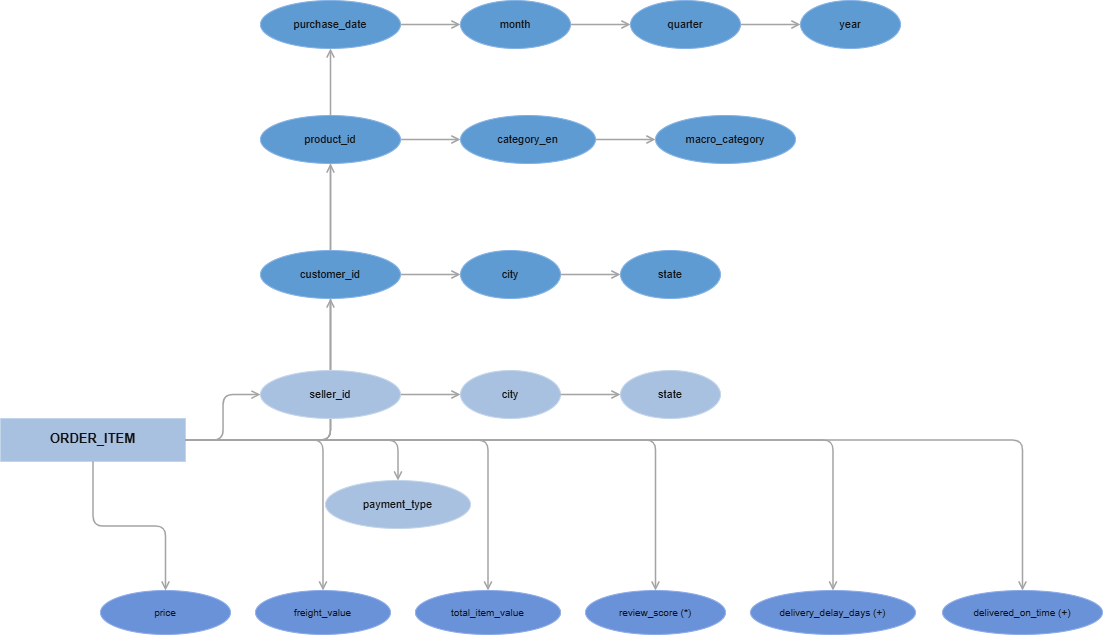
\includegraphics[width=\textwidth]{attribute_tree_pieno.png}
  \caption{Attribute Tree della fact table \texttt{Order\_Items}}
  \label{fig:attrtree}
\end{figure}

\subsection{Dall'Attribute Tree allo Schema DFM}

Partendo dall'attribute tree, ho applicato le regole del metodo data-driven per
ricavare lo schema DFM. I passaggi principali:

\begin{enumerate}
  \item \textbf{Identificazione delle dimensioni}: le chiavi esterne
        (\texttt{product\_id}, \texttt{seller\_id}, \texttt{customer\_id},
        \texttt{payment\_type}, \texttt{purchase\_date}) sono state promosse a
        dimensioni.

  \item \textbf{Editing dell'attribute tree}: secondo la metodologia DFM, l'editing
        dell'albero avviene tramite due operazioni. Il \textbf{pruning} di un vertice
        $v$ consiste nella rimozione dell'intero sottoalbero radicato in $v$: gli
        attributi eliminati non saranno disponibili nella fact table né utilizzabili
        per aggregare i dati. Il \textbf{grafting} di un vertice $v$ con padre $v'$ si
        usa invece quando $v$ esprime un'informazione non interessante ma i suoi
        discendenti vanno mantenuti: i figli di $v$ vengono collegati direttamente a
        $v'$ ed $v$ viene eliminato; si perde così il livello di aggregazione di $v$,
        ma si preservano i livelli sottostanti. Ho applicato queste operazioni come
        segue:
        \begin{itemize}
        \sloppy
          \item \textit{Pruning di \texttt{customer\_unique\_id}}: rimozione
                dell'intero sottoalbero (vertice foglia, senza discendenti). A livello
                di singolo order item, \texttt{customer\_id} è già sufficiente:
                includerlo sarebbe ridondante.
          \item \textit{Grafting di \texttt{zip\_code\_prefix}}: il vertice
                \texttt{zip\_code\_prefix} viene eliminato e i suoi figli
                \texttt{city} e \texttt{state} vengono collegati direttamente al
                padre (\texttt{customer\_id}/\texttt{seller\_id}). Si perde la
                granularità per singolo CAP, troppo fine per le analisi previste, ma
                si preserva la gerarchia geografica $\text{city} \to \text{state}$.
          \item \textit{Pruning degli attributi testo di Reviews}: rimozione
                dell'intero sottoalbero dei campi testuali liberi, non strutturati e
                senza valore per analisi OLAP quantitative. Mantenuto solo
                \texttt{review\_score} come misura.
          \item \textit{Pruning dei flag di qualità}: rimozione dell'intero sottoalbero
                dei flag \texttt{\_imputed}/\texttt{\_outlier}/\texttt{\_missing} --
                utili nel reconciled database per auditing, ma privi di significato
                analitico nel DWH.
          \item \textit{Aggiunta gerarchia \texttt{category\_en} $\to$
                \texttt{macro\_category}}: la sorgente espone solo la categoria in
                portoghese. Ho aggiunto la traduzione in inglese (già disponibile nel
                reconciled database) e una macro-categoria per abilitare operazioni di
                roll-up di alto livello. Non è un'operazione di pruning/grafting in
                senso stretto, ma un'estensione dell'albero con un nuovo attributo
                derivato e una nuova gerarchia.
          \item \textit{Promozione di \texttt{payment\_type} a dimensione}: secondo le
                regole DFM le dimensioni si scelgono tra i figli diretti della radice
                dell'attribute tree. Un ordine può avere più pagamenti (es.\ voucher
                $+$ carta): per evitare duplicazioni nella fact table, ho associato a
                ogni riga il \textbf{metodo di pagamento della prima rata registrata
                per l'ordine} nella tabella dei pagamenti riconciliata
                (\texttt{rec\_fact\_payments}), mentre \texttt{payment\_value}
                rappresenta la somma di tutti gli importi pagati per quell'ordine.
                Si tratta di una scelta deterministica ma non basata sull'importo
                della singola rata: una possibile estensione futura è normalizzare i
                pagamenti multipli in una bridge table dedicata, evitando così la
                scelta di un singolo metodo ``principale''.
          \item \textit{Trattamento di \texttt{total\_item\_value} e
                \texttt{delivered\_on\_time}}: compaiono nell'attribute tree come misure
                concettuali. \texttt{total\_item\_value} $=$ \texttt{price} $+$
                \texttt{freight\_value} non è memorizzata nella fact table perché
                derivabile on-the-fly; viene calcolata direttamente negli strumenti di
                analisi (Tableau). \texttt{delivered\_on\_time} è derivabile da
                \texttt{delivery\_delay\_days} $\leq 0$: non richiede una colonna
                dedicata nel DWH.
        \end{itemize}

  \item \textbf{Gerarchie di roll-up}:
        \begin{itemize}
          \item \textbf{Tempo}: giorno $\to$ mese $\to$ trimestre $\to$ anno
          \item \textbf{Prodotto}: \texttt{product\_id} $\to$ \texttt{category\_en}
                $\to$ \texttt{macro\_category}
          \item \textbf{Cliente}: \texttt{customer\_id} $\to$ \texttt{city} $\to$
                \texttt{state} $\to$ \texttt{region}
          \item \textbf{Venditore}: \texttt{seller\_id} $\to$ \texttt{city} $\to$
                \texttt{state}
          \item \textbf{Pagamento}: \texttt{payment\_type} $\to$
                \texttt{payment\_category}
        \end{itemize}

  \item \textbf{Classificazione delle misure} in base all'additività:
        \begin{itemize}
        \sloppy
          \item \textit{Additive}: \texttt{price}, \texttt{freight\_value} --
                sommabili lungo tutte le dimensioni, incluso il livello item;
          \item \textit{Additive solo a livello ordine}: \texttt{payment\_value},
                \texttt{payment\_installments} -- provengono da un aggregato per
                \texttt{order\_id} (Sezione~\ref{sec:join-fact-sales}) e vengono
                replicate identiche su tutte le righe item dello stesso ordine in
                \texttt{fact\_sales}; \textbf{non sono additive a livello item} (una
                SUM su più item dello stesso ordine duplica il valore). Vanno
                aggregate per \texttt{order\_id} prima di applicare SUM, oppure usate
                con AVG a livello item;
          \item \textit{Non additiva}: \texttt{review\_score} -- solo AVG, la somma
                dei punteggi non ha significato;
          \item \textit{Semi-additive}: \texttt{delivery\_delay\_days},
                \texttt{delivery\_lead\_days} -- non sommabili nel tempo (la somma dei
                ritardi non ha significato), ma aggregabili con AVG, MAX, MIN.
        \end{itemize}
\end{enumerate}

\subsection{Considerazioni sulla perdita di informazione}

Due scelte progettuali comportano una perdita controllata di informazione:

\begin{itemize}
  \item \textbf{Pagamenti multipli}: i pagamenti vengono aggregati per
        \texttt{order\_id} (somma di \texttt{payment\_value} e
        \texttt{payment\_installments}, metodo di pagamento principale) prima del
        join con gli order-item. Si perde il dettaglio dei pagamenti secondari per
        metodo. Inoltre, poiché l'aggregato è per ordine ma viene riportato su ogni
        riga item, \texttt{payment\_value} e \texttt{payment\_installments} sono
        additivi solo a livello ordine, non a livello item (cfr.\
        Sezione~\ref{sec:join-fact-sales} e Tabella~\ref{tab:misure}).
  \item \textbf{Geolocalizzazione}: aggregando per ZIP si perde la variabilità
        puntuale delle coordinate. Accettabile perché le analisi previste lavorano a
        livello città/stato. Da segnalare che 278 record cliente (157 ZIP distinti) e
        7 venditori non
        hanno corrispondenza in \texttt{Geolocation}: per questi record, \texttt{lat}
        e \texttt{lng} risultano NULL nel DWH, senza impatto sulle analisi geografiche
        per stato.
\end{itemize}

Lo schema DFM risultante è in Figura~\ref{fig:dfm}.

\begin{figure}[H]
  \centering
  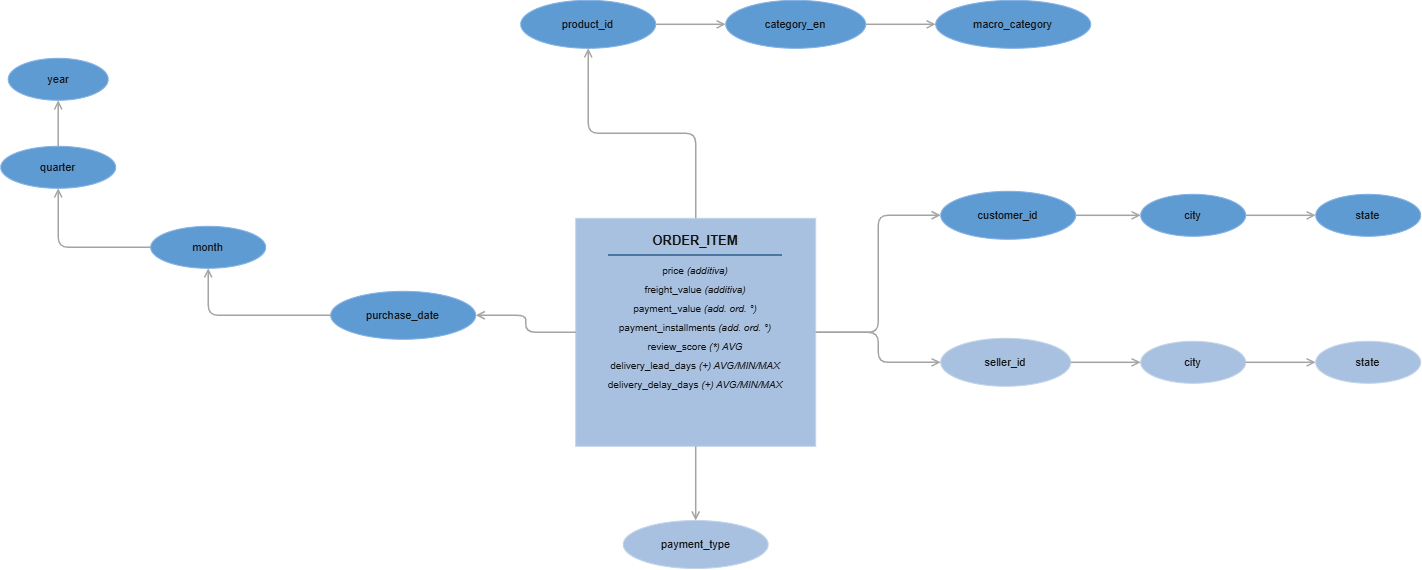
\includegraphics[width=0.85\textwidth]{dfm_schema_pieno_v2.png}
  \caption{Schema DFM del fatto \texttt{ORDER\_ITEM}}
  \label{fig:dfm}
\end{figure}

% ═══════════════════════════════════════════════════════════════════════════
%  5. PROGETTAZIONE LOGICA – STAR SCHEMA
% ═══════════════════════════════════════════════════════════════════════════
\section{Progettazione Logica -- Star Schema}

\subsection{Traduzione dal DFM allo Star Schema}

Ogni dimensione del DFM diventa una tabella con chiave primaria naturale. La fact
table centralizza le FK verso le dimensioni e le misure. La scelta dello \textbf{star
schema} rispetto allo snowflake è motivata dalla semplicità delle query OLAP: meno
join, aggregazioni più veloci. Le gerarchie sono denormalizzate all'interno di
ciascuna tabella di dimensione. Lo schema star è in Figura~\ref{fig:star}.

\begin{figure}[H]
  \centering
  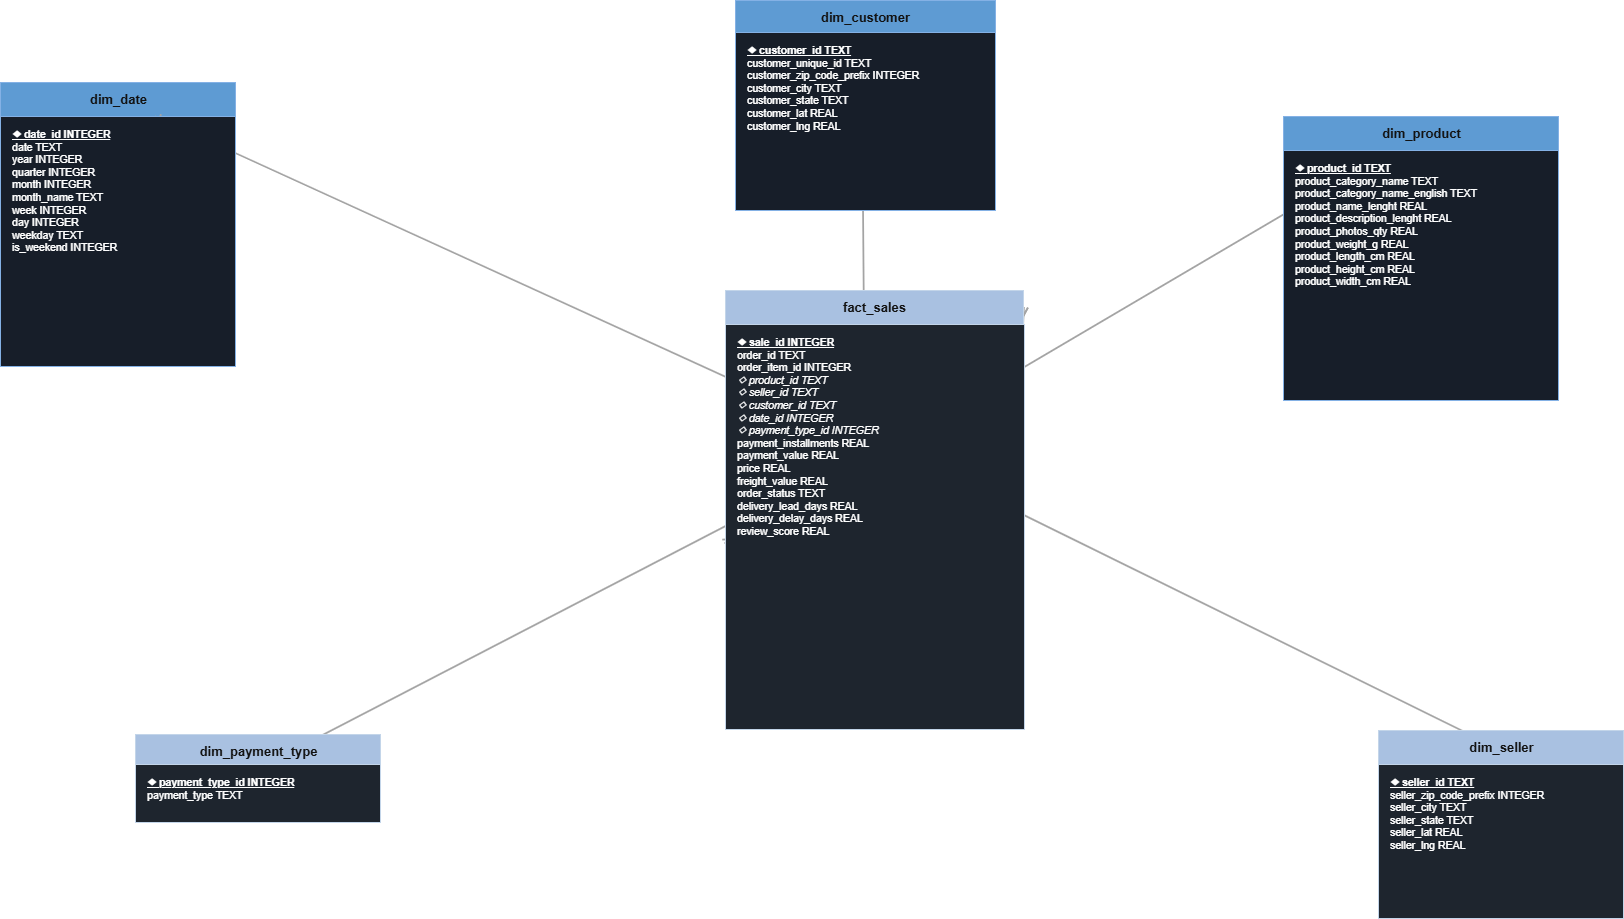
\includegraphics[width=0.85\textwidth]{star_schema_pieno.png}
  \caption{Star Schema del Data Warehouse Olist}
  \label{fig:star}
\end{figure}

\subsection{Supporto alle operazioni OLAP}

Il modello supporta le principali operazioni OLAP:

\begin{itemize}
  \item \textbf{Roll-up}: da giorno a mese, da trimestre ad anno, da città a stato,
        da \texttt{product\_category\_name\_english} a categoria;
  \item \textbf{Drill-down}: da anno a trimestre, da \texttt{category\_en} a singolo
        prodotto;
  \item \textbf{Slice \& Dice}: filtraggio per stato, anno, tipo di pagamento,
        categoria prodotto.
\end{itemize}

\subsection{Tabelle del Data Warehouse}

\begin{table}[H]
  \centering
  \caption{Struttura della fact table \texttt{fact\_sales}}
  \label{tab:fact}
  \begin{tabular}{lll}
    \toprule
    \textbf{Colonna} & \textbf{Tipo} & \textbf{Descrizione} \\
    \midrule
    \texttt{sale\_id}             & INT PK   & Chiave surrogata della fact table \\
    \texttt{order\_id}            & TEXT     & Chiave naturale dell'ordine (tracciabilità) \\
    \texttt{order\_item\_id}      & INT      & Numero progressivo dell'item nell'ordine \\
    \texttt{date\_id}             & INT FK   & Riferimento a \texttt{dim\_date} (YYYYMMDD) \\
    \texttt{product\_id}          & TEXT FK  & Riferimento a \texttt{dim\_product} \\
    \texttt{customer\_id}         & TEXT FK  & Riferimento a \texttt{dim\_customer} \\
    \texttt{seller\_id}           & TEXT FK  & Riferimento a \texttt{dim\_seller} \\
    \texttt{payment\_type\_id}    & INT FK   & Riferimento a \texttt{dim\_payment\_type} \\
    \texttt{order\_status}        & TEXT     & Stato dell'ordine (attributo degenere) \\
    \texttt{payment\_installments} & REAL    & Numero di rate del pagamento -- additiva solo a livello ordine (Tab.~\ref{tab:misure}) \\
    \texttt{price}                & REAL     & Prezzo del prodotto -- misura additiva \\
    \texttt{freight\_value}       & REAL     & Costo di spedizione -- misura additiva \\
    \texttt{payment\_value}       & REAL     & Valore totale del pagamento -- additiva solo a livello ordine (Tab.~\ref{tab:misure}) \\
    \texttt{delivery\_lead\_days} & REAL     & Giorni dalla vendita alla consegna -- semi-additiva (AVG, MAX, MIN) \\
    \texttt{delivery\_delay\_days} & REAL    & Ritardo rispetto alla data stimata (negativo = anticipo) -- semi-additiva \\
    \texttt{review\_score}        & REAL     & Punteggio recensione 1--5 -- solo AVG (non additiva) \\
    \bottomrule
  \end{tabular}
\end{table}

\textit{Nota: \texttt{order\_id} e \texttt{order\_item\_id} sono mantenuti nella fact
table come attributi degeneri per garantire la tracciabilità verso la sorgente
operazionale, senza introdurre una dimensione dedicata. Le misure
\texttt{payment\_value} e \texttt{payment\_installments} provengono da un aggregato
per ordine e sono replicate su ogni riga item: sono quindi additive solo a livello
ordine, non a livello item (cfr.\ Tabella~\ref{tab:misure} e
Sezione~\ref{sec:join-fact-sales}).}

\textbf{Fact table:} \texttt{fact\_sales}

\medskip
\textbf{Tabelle di dimensione}

\underline{\texttt{dim\_date}}(date\_id, date, year, quarter, month, month\_name, week, day, weekday, is\_weekend)\\
\textit{Granularità giornaliera. \texttt{date\_id} = YYYYMMDD (es.\ 20170913).
Supporta roll-up day $\to$ month $\to$ quarter $\to$ year.
634 date distinte per il periodo 2016--2018.}

\medskip
\underline{\texttt{dim\_product}}(product\_id, product\_category\_name,
product\_category\_name\_english, product\_name\_lenght, product\_description\_lenght,
product\_photos\_qty, product\_weight\_g, product\_length\_cm, product\_height\_cm,
product\_width\_cm)\\
\textit{Gerarchia: \texttt{product\_id} $\to$ \texttt{product\_category\_name\_english}.
Nota: il livello \texttt{macro\_category} è previsto nel DFM concettuale ma non
implementato nella versione corrente dello star schema.
I nomi di colonna \texttt{product\_name\_lenght} e \texttt{product\_description\_lenght}
conservano il typo originale della sorgente per compatibilità.}

\medskip
\underline{\texttt{dim\_customer}}(customer\_id, customer\_unique\_id,
customer\_zip\_code\_prefix, customer\_city, customer\_state, customer\_lat, customer\_lng)\\
\textit{Gerarchia geografica: \texttt{city} $\to$ \texttt{state}.
Nota: il livello \texttt{region} è previsto nel DFM concettuale ma non implementato
nella versione corrente.}

\medskip
\underline{\texttt{dim\_seller}}(seller\_id, seller\_zip\_code\_prefix, seller\_city,
seller\_state, seller\_lat, seller\_lng)\\
\textit{Gerarchia geografica: \texttt{city} $\to$ \texttt{state}.}

\medskip
\underline{\texttt{dim\_payment\_type}}(payment\_type\_id, payment\_type)\\
\textit{5 valori: \texttt{credit\_card} (73,9\%), \texttt{boleto} (19,0\%),
\texttt{voucher} (5,6\%), \texttt{debit\_card} (1,5\%), \texttt{not\_defined} (0,003\%).
Collegata alla fact table tramite il metodo di pagamento principale per ogni ordine
(aggregato per \texttt{order\_id}), evitando duplicazioni dovute a ordini con più
metodi di pagamento.}

\subsection{Glossario delle misure}
\label{sec:misure}

\begin{table}[H]
  \centering
  \footnotesize
  \caption{Glossario delle misure della fact table \texttt{fact\_sales}}
  \label{tab:misure}
  \begin{tabular}{>{\ttfamily}l
                  >{\raggedright}p{3.5cm}
                  >{\raggedright\arraybackslash}p{5cm}}
    \toprule
    \textbf{Misura} & \textbf{Tipo / Aggregazione} & \textbf{Descrizione} \\
    \midrule
    price                & Additiva -- SUM, AVG, MIN, MAX &
      Prezzo unitario del prodotto. Sommabile lungo tutte le dimensioni (prodotto,
      cliente, venditore, tempo). \\
    freight\_value       & Additiva -- SUM, AVG &
      Costo di spedizione del singolo item. Sommabile lungo tutte le dimensioni. \\
    payment\_value       & Additiva solo a livello ordine &
      Valore totale del pagamento per l'ordine. \textbf{Attenzione}: in
      \texttt{fact\_sales} è replicato su ogni riga item dello stesso ordine
      (Sezione~\ref{sec:join-fact-sales}); una SUM a livello item sovrastima il
      totale (nel DWH: 19,23M contro 15,38M nei pagamenti originali). Aggregare
      per \texttt{order\_id} prima di sommare, oppure usare AVG a livello item. \\
    payment\_installments & Additiva solo a livello ordine &
      Numero di rate del pagamento, replicato su ogni item dello stesso ordine per
      lo stesso motivo di \texttt{payment\_value}. Aggregare per \texttt{order\_id}
      prima di analisi sull'uso del credito per categoria/area geografica. \\
    delivery\_lead\_days & Semi-additiva -- AVG, MAX, MIN &
      Giorni dalla data di acquisto alla consegna effettiva. Non sommabile nel
      tempo; ha senso aggregare con AVG, MAX, MIN. NULL per ordini non consegnati. \\
    delivery\_delay\_days & Semi-additiva -- AVG, MAX, MIN &
      Ritardo rispetto alla data di consegna stimata (valore negativo = anticipo).
      Non sommabile nel tempo. NULL per ordini non consegnati. \\
    review\_score        & Non additiva -- AVG only &
      Punteggio recensione da 1 a 5. La somma è priva di significato: solo AVG
      è un'aggregazione semanticamente valida. \\
    COUNT(*)             & Conteggio -- SUM &
      Numero di item venduti. Aggregabile lungo tutte le dimensioni; equivale al
      numero di transazioni a livello di granularità. \\
    \bottomrule
  \end{tabular}
\end{table}

\textit{Nota sull'additività:} le misure \texttt{delivery\_delay\_days} e
\texttt{delivery\_lead\_days} sono incluse in \texttt{fact\_sales} come misure
semi-additive: aggregabili con AVG, MAX, MIN ma non con SUM nel tempo.
Risultano NULL per gli ordini non ancora consegnati (null semantico, non dato mancante).

% ═══════════════════════════════════════════════════════════════════════════
%  6. IMPLEMENTAZIONE E POPOLAMENTO (ETL)
% ═══════════════════════════════════════════════════════════════════════════
\section{Implementazione e Popolamento (ETL)}

\subsection{Architettura del processo ETL}

Il passaggio dal reconciled database allo star schema segue il processo ETL
(\textit{Extract, Transform, Load}), eseguito per costruire il database SQLite
finale \texttt{olist\_dw.db}. Questa fase è implementata nello script
\texttt{consegna/2\_scripts/build\_star\_schema.py}, eseguibile a partire dai
CSV puliti in \texttt{consegna/3\_cleaned\_data/}: lo script ricostruisce sia
il reconciled layer (\texttt{rec\_*}) sia il data warehouse layer
(\texttt{dim\_*} e \texttt{fact\_sales}), garantendo la riproducibilità
dell'intero processo descritto in questa sezione (in particolare le regole
di aggregazione di \texttt{payment\_type}/\texttt{payment\_value} discusse in
Sezione~\ref{sec:join-fact-sales}).
L'architettura prevede due livelli distinti nel database SQLite:

\begin{itemize}
  \item \textbf{Reconciled layer} (\texttt{rec\_*}): contiene i dati puliti dal
        notebook di cleaning, caricati direttamente dai CSV. Costituisce il
        \textit{operational data store} dal quale il processo ETL estrae i dati per
        costruire il data warehouse. Mantiene tutte le colonne di audit (flag
        \texttt{\_imputed}, \texttt{\_outlier}) e le misure derivate
        (\texttt{delivery\_delay\_days}, ecc.).
  \item \textbf{Data warehouse layer} (\texttt{dim\_*} + \texttt{fact\_sales}):
        star schema ottimizzato per query OLAP, privo dei flag di qualità e con
        gerarchie denormalizzate nelle dimensioni.
\end{itemize}

Il processo ETL si articola in tre fasi:

\begin{enumerate}
  \item \textbf{Extract}: lettura dei CSV puliti e caricamento nel reconciled layer
        tramite \texttt{pandas.to\_sql()} con \texttt{if\_exists=``replace''}.

  \item \textbf{Transform}: costruzione delle tabelle di dimensione e della fact
        table a partire dal reconciled layer. In particolare:
        \begin{itemize}
          \item Le tabelle \texttt{dim\_*} vengono popolate per prime (no FK violation).
                Le chiavi naturali (\texttt{product\_id}, \texttt{customer\_id}, ecc.\
                ) sono mantenute come chiavi primarie, garantendo tracciabilità.
          \item \texttt{dim\_date} è generata sinteticamente estraendo le date distinte
                dai timestamp di acquisto (\texttt{rec\_orders}), con calcolo di anno,
                mese, trimestre, giorno e giorno della settimana. Copre il periodo
                2016--2018 (634 date distinte).
          \item \texttt{dim\_customer} e \texttt{dim\_seller} sono arricchite con le
                coordinate geografiche (\texttt{lat}/\texttt{lng}) tramite LEFT JOIN
                con \texttt{rec\_geolocation} su \texttt{zip\_code\_prefix}.
          \item \texttt{fact\_sales} viene popolata tramite JOIN tra
                \texttt{rec\_order\_items}, \texttt{rec\_orders}, pagamenti aggregati
                per ordine (\texttt{payment\_value} e \texttt{payment\_installments}
                come somma su tutte le rate, \texttt{payment\_type} come prima rata
                registrata) e media delle
                recensioni per ordine. Le chiavi naturali \texttt{order\_id} e
                \texttt{order\_item\_id} sono mantenute come attributi degeneri.
        \end{itemize}

  \item \textbf{Load}: le tabelle trasformate vengono caricate nel DB finale
        (\texttt{olist\_dw.db}) con vincoli di integrità referenziale abilitati
        (\texttt{PRAGMA foreign\_keys = ON}). Il DB è pronto per essere interrogato
        con strumenti di analisi e visualizzazione (es.\ Tableau, SQLiteViewer).
\end{enumerate}

\subsection{Dettaglio dei JOIN per la costruzione di \texttt{fact\_sales} e delle dimensioni}
\label{sec:join-fact-sales}

La tabella \texttt{fact\_sales} è costruita a partire da \texttt{rec\_order\_items}
(una riga per prodotto per ordine) unendo quattro sorgenti del reconciled layer:

\begin{itemize}
\sloppy
  \item \textbf{JOIN con \texttt{rec\_orders}} su \texttt{order\_id}: porta in
        \texttt{fact\_sales} il \texttt{customer\_id} e il \texttt{date\_id}
        (ricavato convertendo \texttt{order\_purchase\_timestamp} nel formato
        intero YYYYMMDD).

  \item \textbf{LEFT JOIN con i pagamenti pre-aggregati}: prima del join, i
        pagamenti vengono aggregati per \texttt{order\_id}: \texttt{payment\_value}
        e \texttt{payment\_installments} tramite \texttt{SUM} su tutte le rate
        dell'ordine (indipendentemente dal metodo), mentre \texttt{payment\_type}
        viene preso dalla prima rata registrata per l'ordine (\texttt{first()}).
        Il LEFT JOIN garantisce che gli order-item senza pagamento registrato non
        vengano persi.
        \textbf{Effetto collaterale}: per gli ordini con più order-item, il totale
        aggregato per ordine viene replicato su ciascuna riga item di
        \texttt{fact\_sales}. Di conseguenza \texttt{payment\_value} e
        \texttt{payment\_installments} risultano \textit{additivi solo a livello
        ordine} e non a livello item (cfr.\ Tabella~\ref{tab:misure}): la SUM di
        \texttt{payment\_value} sull'intera \texttt{fact\_sales} vale 19,23M contro
        i 15,38M dei pagamenti originali aggregati per ordine.

  \item \textbf{LEFT JOIN con le recensioni pre-aggregate}: le recensioni vengono
        aggregate per \texttt{order\_id} con \texttt{AVG(review\_score)}, in
        quanto un ordine può ricevere più valutazioni. Il LEFT JOIN preserva anche
        gli order-item privi di recensione.
\end{itemize}

Le tabelle di dimensione vengono costruite come segue:

\begin{itemize}
  \item \textbf{\texttt{dim\_customer}} e \textbf{\texttt{dim\_seller}} vengono
        arricchite con le coordinate geografiche (\texttt{lat}/\texttt{lng})
        tramite LEFT JOIN con \texttt{rec\_geolocation} su
        \texttt{zip\_code\_prefix}. Il LEFT JOIN è essenziale: 278 record cliente
        (157 ZIP distinti) e 7 venditori risultano assenti in \texttt{rec\_geolocation}; un INNER
        JOIN eliminerebbe quei record, producendo chiavi orfane in
        \texttt{fact\_sales}.

  \item \textbf{\texttt{dim\_date}} è generata sinteticamente: il codice estrae le
        date distinte da \texttt{rec\_orders.order\_purchase\_timestamp} e calcola
        per ciascuna anno, mese, trimestre, giorno e giorno della settimana. La
        chiave primaria \texttt{date\_id = YYYYMMDD} è un intero ordinabile e
        immediatamente leggibile (es.\ 20170913).

  \item \textbf{\texttt{dim\_payment\_type}} è ricavata dai valori distinti di
        \texttt{payment\_type} presenti in \texttt{rec\_fact\_payments}, ai quali
        viene assegnata una chiave surrogata intera progressiva. Risultano 5 valori:
        \textit{credit\_card}, \textit{boleto}, \textit{voucher},
        \textit{debit\_card}, \textit{not\_defined}.
\end{itemize}

\subsection{Statistiche Finali del Data Warehouse}

\begin{table}[H]
  \centering
  \caption{Volumetrie finali dello Star Schema}
  \label{tab:volumes}
  \begin{tabular}{lrl}
    \toprule
    \textbf{Tabella} & \textbf{Record} & \textbf{Note} \\
    \midrule
    \texttt{fact\_sales}        & 112.650 & Tutte le righe d'ordine con FK operative valide \\
    \texttt{dim\_customer}      &  99.441 & Un record per \texttt{customer\_id} \\
    \texttt{dim\_product}       &  32.951 & Include categoria in inglese \\
    \texttt{dim\_seller}        &   3.095 & Include lat/lng da geolocation \\
    \texttt{dim\_date}          &     634 & Periodo 2016--2018 \\
    \texttt{dim\_payment\_type} &       5 & credit\_card, boleto, voucher, debit\_card, not\_defined \\
    \bottomrule
  \end{tabular}
\end{table}

\textbf{Integrità referenziale}: verificata con query di controllo sul DB finale.
La tabella \texttt{fact\_sales} non presenta righe orfane verso
\texttt{dim\_product}, \texttt{dim\_seller}, \texttt{dim\_customer} e
\texttt{dim\_date}. Per \texttt{payment\_type\_id}: 3 valori NULL legittimi,
corrispondenti alle 3 righe item di un unico ordine (consegnato) per il quale la
sorgente non registra alcun pagamento -- caso noto del dataset Olist; non
costituiscono FK orfane ma riflettono uno stato operativo reale del dataset.

\end{document}
